\documentclass[a4paper,fleqn]{cas-sc}
\usepackage{fontspec}
\setmainfont{Nimbus Roman}[SmallCapsFont={Nimbus Roman}]
\setsansfont{Nimbus Sans}
\setmonofont{Nimbus Mono PS}
\usepackage[authoryear]{natbib}
\usepackage{amsmath,amssymb}
\usepackage{graphicx}
\usepackage{tikz}
\usepackage{pgfplots}
\usepgfplotslibrary{groupplots,fillbetween}
\usetikzlibrary{patterns}
\usetikzlibrary{positioning,fit,arrows.meta}
\usepackage{booktabs}
\usepackage{array}
\usepackage{float}
\usepackage{xcolor}
\usepackage{microtype}
\microtypesetup{expansion=false}
\IfFileExists{xurl.sty}{\usepackage{xurl}}{\usepackage{url}}
\setlength{\emergencystretch}{3em}
\floatstyle{ruled}
\newfloat{algorithm}{tbp}{loa}
\floatname{algorithm}{Алгоритм}
\floatstyle{plain}
\restylefloat{figure}
\restylefloat{table}
\newtheorem{proposition}{Твердження}
\newtheorem{corollary}{Наслідок}
\newdefinition{remark}{Зауваження}
\newproof{proof}{Доведення}
\newcommand{\ibar}{\bar{y}}
\newcommand{\sbar}{\bar{s}}
\newcommand{\Exp}{\mathrm{Exp}}
\newcommand{\Full}{\textup{\textsc{Full}}}
\newcommand{\TS}{\textup{\textsc{TwoScale}}}
\newcommand{\ind}{\mathbf{1}}
\newcommand{\eW}{e_{W}}

\renewcommand{\figurename}{Рисунок}
\renewcommand{\tablename}{Таблиця}
\renewcommand{\refname}{Література}
\RenewDocumentCommand{\keywordtitle}{}{Ключові слова}
\AtBeginDocument{
\newlabel{app:clique}{{A}{25}{}{}{}}
\newlabel{app:floor}{{B}{27}{}{}{}}
\newlabel{app:repro}{{C}{28}{}{}{}}
\newlabel{sec:discussion}{{7}{22}{}{}{}}
\newlabel{tab:verification}{{3}{26}{}{}{}}
}
% BEGIN EDITABLE PLOT STYLE
% Shared plotting style; all text inherits the article font.
\providecommand{\ArrivalCellFont}{\fontsize{6}{7}\selectfont}
\pgfplotsset{compat=1.18,paper axis/.style={font=\scriptsize,label style={font=\scriptsize},title style={font=\small},tick label style={font=\scriptsize},legend style={font=\scriptsize,draw=none,fill=none},axis line style={black!65},tick style={black!65},grid=major,grid style={black!10},scaled ticks=false,unbounded coords=jump,clip=true}}
\definecolor{FullBlue}{HTML}{2878B5}
\definecolor{ScaleOrange}{HTML}{D45A44}
\definecolor{Size50}{HTML}{D73027}
\definecolor{Size100}{HTML}{FC8D59}
\definecolor{Size250}{HTML}{4575B4}
\definecolor{Size1000}{HTML}{313695}
\pgfplotsset{colormap={paperdiv}{rgb=(0.01960784,0.18823529,0.38039216);
rgb=(0.12725875,0.39584775,0.66874279);
rgb=(0.26274510,0.57647059,0.76470588);
rgb=(0.56647443,0.76870434,0.86851211);
rgb=(0.81960784,0.89803922,0.94117647);
rgb=(0.96908881,0.96647443,0.96493656);
rgb=(0.99215686,0.85882353,0.78039216);
rgb=(0.95455594,0.64175317,0.50572857);
rgb=(0.83921569,0.37647059,0.30196078);
rgb=(0.69227220,0.09227220,0.16770473);
rgb=(0.40392157,0.00000000,0.12156863);}}
\pgfplotsset{colormap={paperseq}{rgb=(1.00000000,1.00000000,0.89803922);
rgb=(1.00000000,0.97539408,0.77193387);
rgb=(0.99764706,0.92156863,0.63607843);
rgb=(0.99607843,0.84347559,0.46915802);
rgb=(0.99607843,0.73490196,0.28000000);
rgb=(0.99497116,0.59747789,0.15949250);
rgb=(0.93960784,0.47137255,0.09490196);
rgb=(0.84822760,0.35229527,0.03497116);
rgb=(0.72000000,0.26039216,0.01098039);
rgb=(0.55686275,0.19123414,0.01737793);
rgb=(0.40000000,0.14509804,0.02352941);}}
% END EDITABLE PLOT STYLE
\begin{document}
\let\WriteBookmarks\relax
\shorttitle{Двомасштабне стохастичне моделювання з агрегованим міжспільнотним зв'язком}
\shortauthors{Y. Kuryliak and M.T.M. Emmerich}

\title[mode=title]{Двомасштабне стохастичне моделювання епідемій у мережах спільнот з агрегованим міжспільнотним зв'язком}

\author[1]{Yulian Kuryliak}[orcid=0000-0002-6600-2637]
\cormark[1]
\ead{yulian.a.kuryliak@lpnu.ua}
\affiliation[1]{organization={Інститут комп'ютерних наук та інформаційних технологій, Національний університет ``Львівська політехніка''},
            addressline={вул. Степана Бандери, 12},
            city={Львів},
            postcode={79000},
            country={Україна}}

\author[2]{Michael T. M. Emmerich}[orcid=0000-0002-7342-2090]
\ead{michael.t.m.emmerich@jyu.fi}
\affiliation[2]{organization={Факультет інформаційних технологій, Університет Ювяскюля},
            addressline={P.O. Box 35 (Agora)},
            city={Ювяскюля},
            postcode={FI-40014},
            country={Фінляндія}}

\cortext[1]{Автор для листування}


% Попередня анотація; розділи з результатами ще не включено.
\begin{abstract}
Для стохастичного моделювання поширення епідемій у великих
контактних мережах часто бракує інформації про конкретні
контакти між людьми. Водночас можуть бути доступні
агреговані дані про переміщення населення та зв'язки між
містами чи іншими спільнотами. Внутрішні контактні мережі
спільнот можна наближено відтворювати за відомими
структурними характеристиками, проте конкретні контакти
між ними залишаються невідомими. У роботі досліджено
двомасштабний метод стохастичного моделювання (\TS{}),
який поєднує детальні локальні симулятори Gillespie
з агрегованими міжспільнотними інтенсивностями
передавання інфекції без явного представлення
міжспільнотних контактів.

Теоретично доведено, що ідеальний двомасштабний процес
еквівалентний точному моделюванню на сурогатній мережі
з рівномірно розподіленими міжспільнотними зв'язками.
Визначено механізми розбіжностей із повномережевою
моделлю та встановлено стохастично не пізніший
час першого експорту інфекції за рівномірного
випадкового розміщення вузлів-мостів у розглянутій
теоретичній постановці.

Точність методу досліджено шляхом порівняння
з повномережевим Gillespie на синтетичних SI-мережах,
зокрема у 48 конфігураціях ланцюгів із десяти
спільнот. Експерименти продемонстрували близькість
часових розподілів за швидкого внутрішнього поширення:
у ланцюгу десяти клік нормована відстань Вассерштайна
після дев'яти міжспільнотних переходів становила
$3.34\%$. Встановлено залежність розбіжностей
від структури й розміру спільнот, кількості
міжспільнотних ребер та співвідношення часових
масштабів внутрішнього й міжспільнотного поширення.
Запропонований показник цього співвідношення
продемонстрував сильний ранговий зв'язок із величиною
розбіжностей (кореляція Спірмена $0.91$).

Результати підтверджують можливість відтворення
близьких до повномережевого моделювання часових
характеристик без знання конкретної структури
міжспільнотних контактів та допомагають визначати
умови, за яких таке наближення є доцільним.
\end{abstract}

\begin{keyword}
Стохастичне моделювання епідемій
\sep Алгоритм Gillespie
\sep Багатомасштабне моделювання
\sep Мережі спільнот
\sep Агреговані міжспільнотні зв'язки
\sep Неповні контактні дані
\sep Точність моделювання
\end{keyword}
\maketitle
% Простіший чорний текст розділів 1--3; основа — узгоджена parallel-версія.

\section{Вступ}
\label{sec:introduction}

Епідемія поширюється на кількох рівнях. Усередині спільноти зараження може залежати від конкретних контактів між людьми \citep{keeling2005,pastorsatorras2015,kiss2017}. Для зв'язків між спільнотами дані часто менш докладні: наприклад, відома лише кількість пасажирів, обсяг поїздок на роботу або загальна вага зв'язку між двома місцями \citep{balcan2009,barbosa2018human}. Тому потрібна модель, яка поєднує докладну контактну мережу всередині кожної спільноти із загальними даними про зв'язки між спільнотами.

Така ситуація виникає на практиці. Локальну контактну мережу можна спостерігати, відновлювати або генерувати за відомими характеристиками, зокрема кластеризацією та середньою довжиною найкоротших шляхів \citep{eubank2004,danon2011}. Натомість зв'язки між спільнотами можуть бути відомі лише з транспортних, міграційних даних, даних про поїздки на роботу чи даних мобільних операторів \citep{barbosa2018human,chang2021}. Вони дають загальну силу зв'язку, але не визначають людей, через яких інфекція може перейти між спільнотами. Отже, ми можемо знати вагу зв'язку, не знаючи конкретних вузлів-мостів та їхнього стану.

Якщо відомі всі контакти, епідемію можна описати неперервним марковським ланцюгом (CTMC) і точно моделювати методом Gillespie \citep{gillespie1977exact,gibson2000}. Є також ефективні методи для часових, великих і розріджених мереж \citep{vestergaard2015,kuryliak2025simulating}. Проте їм усе одно потрібні конкретні контакти, здатні передавати інфекцію. Метапопуляційні моделі використовують загальні потоки між спільнотами, але зазвичай замінюють і докладну локальну мережу кількостями людей у різних станах \citep{colizza2007reaction,colizza2008,balcan2010modeling,ajelli2010}. Наша задача лежить між цими двома випадками: зберегти випадкове поширення між окремими вузлами всередині спільнот, використовуючи лише загальні дані для зв'язків між ними.

Ідею двомасштабного симулятор представлено в попередній конференційній роботі \citep{kuryliak2025towards}. Для кожної спільноти він запускає окремий локальний симулятор. Макрорівень використовує поточні стани спільнот і ваги зв'язків, щоб генерувати зараження, які надходять з іншої спільноти. У цій статті ми докладно описуємо метод і досліджуємо його похибку. Зокрема, з'ясовуємо, що втрачається, коли справжні міжспільнотні ребра та їхні кінцеві вузли замінено загальною вагою зв'язку, а імпортоване зараження потрапляє на випадково вибраний сприйнятливий вузол.

Головне питання: коли такого агрегованого зв'язку достатньо для відтворення потрібної нам характеристики повномережевого CTMC? Ми досліджуємо часи прибуття інфекції, їхні розподіли та можливість передавання через справжні контакти. Близькі часи ще не гарантують можливого шляху
передавання: двомасштабна модель може заразити іншу спільноту, поки всі справжні вузли-мости в спільноті-
джерелі ще сприйнятливі. Для перевірки ми використовуємо синтетичні мережі, у яких відомі всі контакти.
Повний Gillespie отримує всю мережу, а двомасштабний метод — лише локальні мережі та загальні ваги
міжспільнотних зв’язків.

Стаття має чотири основні результати.
\begin{enumerate}
\item Описуємо, як працює симулятор: кожна спільнота моделюється окремо, а спільний планувальник визначає
зараження між ними. Пояснюємо, як він узгоджує локальні симулятори на часових інтервалах фіксованої довжини (Розділ~\ref{sec:method}, Алгоритм~\ref{alg:scheduler}).
\item Показуємо, яку мережу метод моделює точно. Ідеальний процес точний для \emph{сурогатної мережі з рівномірними міжспільнотними зв’язками}: між кожними двома зв’язаними спільнотами всі вузли однієї з’єднано з усіма вузлами іншої, а загальну вагу зв’язку розподілено порівну між цими парами (Твердження~\ref{prop:surrogate}). Далі ми визначаємо джерела похибки та аналізуємо один експорт інфекції (Твердження~\ref{prop:ordering}).
\item Ми порівнюємо двомасштабний метод із повномережевим моделюванням Gillespie для передавання інфекції в одну сусідню спільноту та її поширення вздовж ланцюга спільнот. Відмінності оцінюємо за відносним зсувом медіани часу першого зараження та відстанню Вассерштайна між розподілами цих часів.  (Розділи~\ref{sec:design} і~\ref*{sec:results}).
\item Ми пропонуємо емпіричний показник точності для наших тестів. Він порівнює розкид часів зараження всередині спільноти з типовим часом передавання через одне міжспільнотне ребро (Розділ~\ref*{sec:res_descriptor}).
\end{enumerate}

Ми розглядаємо динаміку «сприйнятливий--інфікований» (SI) на статичних синтетичних мережах і використовуємо один фіксований крок синхронізації. Розділ~\ref{sec:related} пояснює зв'язок із попередніми методами. Розділ~\ref{sec:method} описує симулятор. У Розділі~\ref{sec:analysis} пояснено, яку інформацію агрегований зв'язок зберігає та втрачає. Розділи~\ref{sec:design} і~\ref*{sec:results} містять експерименти та результати. У Розділі~\ref*{sec:discussion} обговорено застосування, обчислювальні витрати й обмеження.

\section{Пов'язані праці}
\label{sec:related}

\paragraph{Моделювання випадкових подій.}
Прямий метод Gillespie вибирає наступну подію та її час за поточними інтенсивностями подій \citep{gillespie1977exact}. Метод наступної реакції підтримує окремий годинник для кожної можливої події \citep{gibson2000}. Обидва методи точні для CTMC, який вони моделюють. Якщо інтенсивність змінюється з часом, її можна накопичувати до досягнення випадкового порога \citep{ethier1986}. \citet{anderson2007} використав цю ідею для систем зі змінними інтенсивностями та затримками. Наш макрогодинник працює за тією самою ідеєю, але його інтенсивність змінюється разом зі станами локальних епідемій. Мережеві симулятори можуть зменшувати обсяг роботи, оновлюючи лише інтенсивності, на які вплинула остання подія \citep{vestergaard2015,kuryliak2025simulating}. Наші локальні симулятори використовують реалізацію з \citet{kuryliak2025simulating}.

Деякі багатомасштабні методи прискорюють моделювання хімічних реакцій, наближено описуючи реакції, що відбуваються значно частіше за інші \citep{haseltine2002,cao2005slow}. Наш метод прибирає іншу інформацію. Він зберігає локальні зараження, але не знає, які саме міжспільнотні ребра зараз здатні передавати інфекцію. Попри цю відмінність, співвідношення швидкостей локального поширення та міжспільнотного передавання допомагає пояснити похибку.

\paragraph{Моделі з кількома спільнотами.}
Метапопуляційні моделі описують кожну підпопуляцію кількостями людей у різних станах і зв'язують підпопуляції потоками мобільності. Їх використовували для дослідження глобального поширення та умов проникнення інфекції \citep{colizza2007reaction,colizza2008,balcan2009,balcan2010modeling}. Докладні дані мобільності також можна поєднувати з локальними моделями передавання \citep{chang2021}. Агентні моделі, своєю чергою, представляють окремих людей у всій системі \citep{eubank2004,kerr2021}. \citet{ajelli2010} порівняли ці два підходи. Досліджуваний тут метод зберігає окремі вузли та контакти всередині спільноти, але замінює невідомі індивідуальні контакти між спільнотами одним агрегованим стохастичним зв'язком.

\paragraph{Два рівні перемішування та спільне моделювання.}
Деякі епідемічні моделі поєднують контакти в малих локальних групах із рівномірним перемішуванням на ширшому рівні \citep{ball1997}. Наша сурогатна мережа з рівномірними міжспільнотними зв’язками має подібну ідею, але рівномірне перемішування діє лише між зв'язаними парами спільнот, а його силу визначає загальна вага зв'язку.

Реалізація також має риси спільного моделювання (co-simulation). У ньому окремі симулятори підсистем рухаються вперед за спільною часовою сіткою та обмінюються обмеженим набором даних \citep{gomes2018cosim}. У нас цими підсистемами є локальні симулятори спільнот. Вони передають макрорівню кількості інфікованих і сприйнятливих вузлів. Макрорівень використовує ці дані, щоб згенерувати час міжспільнотного зараження та вибрати спільноту-одержувача й цільовий вузол. Отже, локальні симулятори можуть залишатися «чорними скриньками» для планувальника. У цій реалізації дані, якими вони обмінюються, використовуються для створення випадкових подій зараження.

\section{Метод двомасштабного моделювання}
\label{sec:method}

В експериментах використано одну реалізацію двомасштабного симулятора, для якої локальні симулятори обмінюються з планувальником макро рівня через фіксовані проміжки часу. Щоб зрозуміти її похибку, ми також розглядаємо процес із тими самими інтенсивностями, але з точним визначенням часу кожної події. Цей теоретичний опис називаємо \emph{ідеальним процесом}. Він дає змогу відокремити похибку заміни мережі від додаткової похибки часової сітки. Ідеальний процес точний для сурогатної мережі з рівномірними міжспільнотними зв’язками, визначеної далі; це не означає точності для початкової фізичної мережі. Нижче пояснимо еталонну модель, доступні дані та кроки реалізованого симулятора.

\subsection{Повномережева еталонна модель}
\label{sec:reference}

Нехай $G=(V,E)$ --- контактна мережа. Її вузли поділено на $M$ спільнот, які не перетинаються:
\begin{equation}
\label{eq:partition}
V=V_1\cup V_2\cup\cdots\cup V_M,
\qquad N_i=|V_i|.
\end{equation}
Тут $V_i$ --- множина вузлів спільноти $i$, а $N_i$ --- кількість її вузлів. Позначаємо через $E_{ii}$ контакти всередині спільноти $i$, а через $E_{ij}$ --- контакти від вузлів спільноти $i$ до вузлів спільноти $j$. Контакт представляємо як напрямлений канал передавання. Тому ненапрямлений контакт дає два канали --- по одному в кожному напрямку.

Кожен вузол є сприйнятливим ($S$), інфікованим ($I$) або видаленим ($R$). Повний стан мережі в час $t$ позначаємо $X(t)$, а стан спільноти $i$ --- $X_i(t)$. Множини сприйнятливих та інфікованих вузлів цієї спільноти позначаємо $S_i(t)$ та $I_i(t)$. Їхні кількості --- $s_i(t)$ та $y_i(t)$, а частки --- $\sbar_i(t)=s_i(t)/N_i$ та $\ibar_i(t)=y_i(t)/N_i$. Далі $x$ означає конкретний стан мережі; $x^{v:I}$ --- той самий стан після зараження вузла $v$, а $x^{u:R}$ --- після видалення вузла $u$.

Повна модель має два прості правила переходів між станами. Сприйнятливий вузол $v$ отримує інфекцію від кожного інфікованого сусіда $u$ з інтенсивністю $\beta_{uv}$. Інфікований вузол видаляється з інтенсивністю $\gamma$. Для вузлів у відповідних станах:
\begin{equation}
\label{eq:full_generator}
q_v(x)=\sum_{\substack{u:(u,v)\in E\\x_u=I}}\beta_{uv}
\quad (x_v=S),
\qquad r_u(x)=\gamma\quad (x_u=I).
\end{equation}
Тут $q_v$ --- сумарна інтенсивність зараження вузла $v$, а $r_u$ --- інтенсивність видалення вузла $u$. Для несприйнятливого вузла $q_v=0$; для неінфікованого вузла $r_u=0$. Інтенсивність визначає частоту події: наприклад, за сталої інтенсивності $q$ середній час очікування дорівнює $1/q$.  Для міжспільнотного каналу записуємо $\beta_{uv}=\beta_{\mathrm{out}}w_{uv}$, де $w_{uv}$ --- вага контакту. Точне моделювання цих повномережевих інтенсивностей позначаємо \Full{}. Усі експерименти в статті мають динаміку SI, тобто $\gamma=0$.

Час переходу між станами є експоненційним і визначається сумарною інтенсивністю всіх подій у поточному стані $x$, яка дорівнює
\[
a(x)=\sum_v q_v(x)+\sum_u r_u(x).
\]
Якщо $a(x)>0$, час до наступної події має експоненційний розподіл із параметром $a(x)$ і середнім $1/a(x)$.
Зараження вузла $v$ вибирається з імовірністю $q_v(x)/a(x)$, а видалення вузла $u$ --- з імовірністю $r_u(x)/a(x)$.
Після події інтенсивності перераховуються.
Якщо $a(x)=0$, подальших подій немає.

\subsection{Агрегований інтерфейс}
\label{sec:interface}

Двомасштабний симулятор \TS{} знає кожен локальний граф $G_i=(V_i,E_{ii})$ та його інтенсивності. Він не знає конкретних міжспільнотних каналів у $E_{ij}$. Для кожної напрямленої пари спільнот йому відома лише загальна вага:
\begin{equation}
\label{eq:weight}
W_{ij}=\sum_{(u,v)\in E_{ij}}w_{uv},\qquad i\neq j.
\end{equation}
Якщо всі ваги дорівнюють одиниці, $W_{ij}$ --- кількість каналів від $V_i$ до $V_j$. У прикладній задачі цю величину можна оцінити за транспортними, міграційними даними, даними мобільності або контактів. Макрорівень також отримує поточні кількості сприйнятливих та інфікованих вузлів від кожного локального симулятора. Він не знає, які вузли є кінцями справжніх міжспільнотних ребер. Основні відмінності наведено в Таблиці~\ref{tab:information}; Рисунок~\ref{fig:schematic} показує їх на схемі.

\begin{table}[tbp]
\color{black}\centering
\caption{\textcolor{black}{Дані та правила двох моделей. В усіх експериментах \TS{} вибирає цільовий вузол рівномірно серед сприйнятливих вузлів.}}
\label{tab:information}
\small
\begin{tabular}{>{\raggedright\arraybackslash}p{0.42\linewidth}>{\raggedright\arraybackslash}p{0.23\linewidth}>{\raggedright\arraybackslash}p{0.25\linewidth}}
\toprule
Дані або дія & \Full{} & \TS{}\\
\midrule
Локальні контакти, інтенсивності та стани вузлів & відомі & відомі локальним симуляторам\\
Конкретні міжспільнотні ребра та вузли-мости & відомі & невідомі\\
Загальна міжспільнотна вага $W_{ij}$ & отримана з ребер & задана безпосередньо\\
Інтенсивність міжспільнотного зараження & зі станів кінців справжніх ребер & з $\ibar_i$, $\sbar_j$ та $W_{ij}$\\
Цільовий вузол зараження & кінець ребра, яке передало інфекцію & сприйнятливий вузол, вибраний за правилом\\
Кількість можливих SI-заражень через набір каналів & не більше кількості каналів & не більше $s_j$ цільових заражень\\
\bottomrule
\end{tabular}
\end{table}

\begin{figure}[tbp]
\color{black}\centering
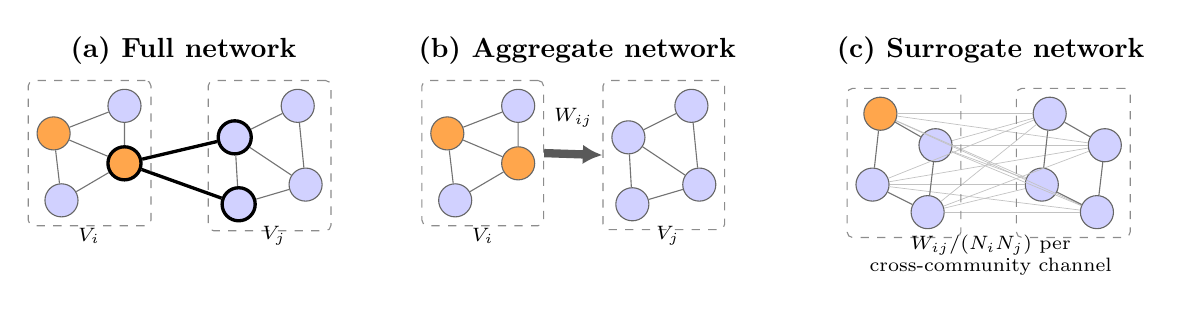
\begin{tikzpicture}[
  x=1cm,y=1cm,
  font=\scriptsize,
  >=Latex,
  person/.style={circle,draw=black!60,fill=blue!18,minimum size=4.2mm,inner sep=0pt},
  infected/.style={person,fill=orange!70},
  bridge/.style={person,very thick,draw=black},
  bridgeinf/.style={infected,very thick,draw=black},
  commbox/.style={draw=black!45,dashed,rounded corners=2pt,inner sep=3pt},
  macrobox/.style={draw=black!70,rounded corners=2pt,fill=black!5,align=center,inner sep=3pt},
  link/.style={draw=black!55},
  weak/.style={draw=black!24,line width=.25pt},
  flow/.style={-{Latex[length=1.7mm]},draw=black!65}
]
% (a) Full microscopic interface
\node[font=\bfseries] at (0,2.25) {(a) Full network};
\node[infected] (a1) at (-1.65,1.20) {};
\node[person]   (a2) at (-1.55,0.35) {};
\node[bridgeinf](a3) at (-0.75,0.82) {};
\node[person]   (a4) at (-0.75,1.55) {};
\node[bridge]   (b1) at (0.65,1.15) {};
\node[person]   (b2) at (1.45,1.55) {};
\node[person]   (b3) at (1.55,0.55) {};
\node[bridge]   (b4) at (0.70,0.30) {};
\draw[link] (a1)--(a2)--(a3)--(a1) (a1)--(a4)--(a3);
\draw[link] (b1)--(b2)--(b3)--(b4)--(b1) (b1)--(b3);
\draw[very thick] (a3)--(b1);
\draw[very thick] (a3)--(b4);
\node[commbox,fit=(a1)(a2)(a3)(a4)] {};
\node[commbox,fit=(b1)(b2)(b3)(b4)] {};
\node at (-1.2,-0.10) {$V_i$};
\node at (1.15,-0.10) {$V_j$};

% (b) Aggregate community network with local contacts retained
\node[font=\bfseries] at (5.0,2.25) {(b) Aggregate network};
\node[infected] (e1) at (3.35,1.20) {};
\node[person]   (e2) at (3.45,0.35) {};
\node[infected] (e3) at (4.25,0.82) {};
\node[person]   (e4) at (4.25,1.55) {};
\node[person]   (f1) at (5.65,1.15) {};
\node[person]   (f2) at (6.45,1.55) {};
\node[person]   (f3) at (6.55,0.55) {};
\node[person]   (f4) at (5.70,0.30) {};
\draw[link] (e1)--(e2)--(e3)--(e1) (e1)--(e4)--(e3);
\draw[link] (f1)--(f2)--(f3)--(f4)--(f1) (f1)--(f3);
\node[commbox,fit=(e1)(e2)(e3)(e4)] (agg_i) {};
\node[commbox,fit=(f1)(f2)(f3)(f4)] (agg_j) {};
\draw[-{Latex[length=2.5mm,width=2.5mm]},draw=black!65,line width=3pt]
      (agg_i.east) -- node[above=5pt,text=black] {$W_{ij}$} (agg_j.west);
\node at (3.8,-0.10) {$V_i$};
\node at (6.15,-0.10) {$V_j$};

% (c) Surrogate interface
\node[font=\bfseries] at (10.25,2.25) {(c) Surrogate network};
\node[infected] (c1) at (8.85,1.45) {};
\node[person]   (c2) at (8.75,0.55) {};
\node[person]   (c3) at (9.55,1.05) {};
\node[person]   (c4) at (9.45,0.20) {};
\node[person]   (d1) at (11.00,1.45) {};
\node[person]   (d2) at (10.90,0.55) {};
\node[person]   (d3) at (11.70,1.05) {};
\node[person]   (d4) at (11.60,0.20) {};
\foreach \u in {c1,c2,c3,c4}{\foreach \v in {d1,d2,d3,d4}{\draw[weak] (\u)--(\v);}}
\draw[link] (c1)--(c2)--(c4)--(c3)--(c1);
\draw[link] (d1)--(d2)--(d4)--(d3)--(d1);
\node[commbox,fit=(c1)(c2)(c3)(c4)] {};
\node[commbox,fit=(d1)(d2)(d3)(d4)] {};
\node[align=center] at (10.25,-0.35) {$W_{ij}/(N_iN_j)$ per\\cross-community channel};
\end{tikzpicture}
\caption{\textcolor{black}{Три подання зв'язку між спільнотами. (a) У повній мережі інфекція переходить лише через показані фізичні ребра та їхні вузли-мости. (b) Усередині кожної спільноти збережено вузли та локальні контакти. Окремі міжспільнотні контакти подано одним широким напрямленим ребром між $V_i$ та $V_j$ із загальною вагою $W_{ij}$. (c) Ідеальний двомасштабний процес еквівалентний процесу на сурогатній мережі з рівномірними міжспільнотними зв’язками: між кожними двома зв’язаними спільнотами всі напрямлені пари вузлів мають однакову вагу контакту. Загальна вага всіх цих зв'язків дорівнює $W_{ij}$. Помаранчеві вузли --- інфіковані, сині --- сприйнятливі.}}
\label{fig:schematic}
\end{figure}

\subsection{Локальні симулятори}
\label{sec:local}

Кожна спільнота має окремий симулятор Gillespie для свого графа $G_i$. Він застосовує інтенсивності зараження та видалення з~\eqref{eq:full_generator}, використовуючи лише локальні ребра $E_{ii}$. Реалізація оновлює лише ті інтенсивності, на які вплинула остання подія, як у \citet{kuryliak2025simulating}. Кожен локальний симулятор є незалежним і має власний потік випадкових чисел.

Макрорівень може просунути локальний симулятор до заданого часу. Симулятор виконує локальні події до цього моменту. Потім макрорівень може імпортувати інфекцію, змінивши стан вибраного сприйнятливого вузла на $I$. Це змінює локальні інтенсивності. Реалізація зберігає невикористану частину випадкового порога наступної локальної події та перераховує час очікування за новою сумарною інтенсивністю. 

Щоб перерахувати час наступної локальної події після імпорту, симулятор зберігає залишок випадкового порога. Нехай $E_{\mathrm{loc}}\sim\mathrm{Exp}(1)$ --- поріг,
згенерований після попередньої локальної події, а
$A_{\mathrm{loc}}$ --- інтеграл сумарної локальної
інтенсивності від тієї події до моменту імпорту.
Після імпорту сумарна локальна інтенсивність
дорівнює $a_{\mathrm{new}}$. Якщо $a_{\mathrm{new}}>0$,
залишковий час очікування становить
\[
\Delta t=
\frac{E_{\mathrm{loc}}-A_{\mathrm{loc}}}{a_{\mathrm{new}}}.
\]
Отже, імпорт змінює час очікування, але не сам випадковий
поріг. Якщо раніше відбудеться ще один імпорт, накопичену
інтенсивність оновлюють і час очікування знову
перераховують. Якщо $a_{\mathrm{new}}=0$, локальна подія
не може відбутися, доки інтенсивність не стане додатною.

Тип події та її вузол вибираються за оновленими інтенсивностями. Новий локальний поріг генерується лише тоді, коли збереженого порога немає. Кожен локальний годинник має власний поріг, окремий від макропорога, описаного в Розділі~\ref{sec:timing}. За заданих часів імпорту та цільових вузлів локальний симулятор виконує правила CTMC своєї мережі. Наближення виникає через спосіб генерування імпортів і вибору їхніх цільових вузлів.

\subsection{Макрорівень}
\label{sec:macro}

Макрорівень представляє спільноту її поточними частками вузлів, а напрямлений зв'язок --- вагою $W_{ij}$. Інтенсивність зараження зі спільноти $i$ до спільноти $j$:
\begin{equation}
\label{eq:macro_rate}
\lambda_{ij}(t)=\beta_{\mathrm{out}}W_{ij}\ibar_i(t)\sbar_j(t),
\qquad \Theta(t)=\sum_{i\neq j}\lambda_{ij}(t).
\end{equation}
Кожен множник має простий зміст. $\beta_{\mathrm{out}}W_{ij}$ задає загальну силу зв'язку; $\ibar_i$ --- частку інфікованих у спільноті-джерелі; $\sbar_j$ --- частку сприйнятливих у спільноті-одержувачі. Сума $\Theta$ --- інтенсивність будь-якого міжспільнотного зараження. Обчислення часу до наступної події, за умови що $\Theta$ змінна в часі, має певні особливості (див \ref{sec:timing}).

Коли така подія відбувається, спочатку вибирають спільноту-джерело та спільноту-одержувача $(i,j)$ з імовірністю $\lambda_{ij}/\Theta$. Потім у спільноті $j$ рівномірно вибирають один сприйнятливий вузол і заражають його. Якщо таких вузлів 20, кожен має імовірність $1/20$. Вибір не враховує справжні вузли-мости, оскільки агрегований інтерфейс їх не знає. У подальших формулах цю імовірність позначаємо $\Pi_{ij}(v\mid x)=1/s_j$ для $v\in S_j$, де $x$ --- поточний стан мережі. Отже, $\Pi$ просто позначає імовірність вибору конкретного сприйнятливого вузла. Інші правила можливі, якщо є інформація про вузли-мости. 

Ця агрегована інтенсивність загалом наближено описує передавання через справжні фізичні ребра. Для заданих кількостей вузлів у станах вона дорівнює очікуваній інтенсивності за рівномірного випадкового вибору кінців ребер, перш ніж враховано їхні конкретні ідентичності, стани та історію епідемії. Це не гарантує правильної інтенсивності для вже реалізованої епідемії на конкретних ребрах. Для рівномірного зв'язку «усі з усіма» вона є фактичною інтенсивністю, як пояснено в Розділі~\ref{sec:analysis}. 

\subsection{Час подій та синхронізація}
\label{sec:timing}

Після макроподії в час $t_0$ генеруємо випадковий поріг $E\sim\Exp(1)$: експоненційне випадкове число із сподіванням один. Починаючи з нуля, накопичуємо загальну інтенсивність $\Theta$:
\begin{equation}
\label{eq:hazard_integral}
A(t)=\int_{t_0}^{t}\Theta(s)\,ds,
\qquad A(t_0)=0.
\end{equation}
Наступна макроподія відбувається в перший момент
$t^\ast$, коли $A(t^\ast)=E$.


Інакше кажучи, площа під кривою інтенсивності зростає до випадкового порога. Якщо поріг не досягнуто, наступної макроподії немає. Це стандартний спосіб визначення часу події за накопиченою інтенсивністю \citep{ethier1986,anderson2007}. За сталої $\Theta$ час очікування дорівнює $E/\Theta$. Якщо згенерувати $E=-\ln U$, де $U$ рівномірно розподілене на $(0,1)$, отримуємо звичний час очікування Gillespie. Коли локальна подія змінює $\Theta$, зберігаємо той самий поріг і продовжуємо накопичення з новою інтенсивністю. Новий макропоріг генеруємо лише після макроподії. Точне визначення першого досягнення порога задає ідеальний процес; описаний нижче розрахунок на часовій сітці наближено визначає цей момент. У Розділі~\ref{sec:surrogate} показано, що ідеальний процес точний для сурогатної мережі з рівномірними міжспільнотними зв’язками.

Планувальник ділить час на інтервали довжини $\tau$.
На кожному інтервалі він наближено замінює змінну
макроінтенсивність її значенням у середині інтервалу. Нехай $A$ --- уже накопичена величина від попередньої макроподії. Для поточного інтервалу $[t,t_g)$ копіюємо кожен локальний симулятор разом зі станом генератора випадкових чисел і просуваємо копію до середини інтервалу. За копіями обчислюємо оцінку загальної макроінтенсивності $\Theta_{\mathrm{mid}}$. Оцінений приріст за залишок інтервалу дорівнює $\Theta_{\mathrm{mid}}(t_g-t)$. Якщо $A$ плюс цей приріст менше за $E$ (випадковий макропоріг), справжні симулятори просуваються до $t_g$. Інакше час події оцінюємо як
\begin{equation}
\label{eq:interpolation}
t^\ast=t+\frac{E-A}{\Theta_{\mathrm{mid}}}.
\end{equation}
Тут $E$ --- випадковий макропоріг, а $A$ --- уже накопичена до нього величина. Чисельник $E-A$ --- залишок до порога; ділення на оцінену інтенсивність дає залишковий час очікування. Наприклад, за $E=1$, $A=0.4$ та $\Theta_{\mathrm{mid}}=0.2$ оцінений час очікування дорівнює трьом одиницям часу. Планувальник просуває справжні симулятори до $t^\ast$, за їхніми станами в цей момент вибирає спільноту-джерело та спільноту-одержувача, вибирає сприйнятливий цільовий вузол і застосовує зараження. Повну послідовність наведено в Алгоритмі~\ref{alg:scheduler}.

\begin{algorithm}[tbp]
\color{black}
\caption{\textcolor{black}{Один запуск двомасштабного симулятора з узгодженням за часовою сіткою.}}
\label{alg:scheduler}
\small

\textbf{Вхід:} локальні графи $G_i$, ваги $W_{ij}$, інтенсивності, крок $\tau$, горизонт $T_{\mathrm{end}}$ та початковий стан.
\begin{enumerate}
\item Установити $t=0$ і $A=0$; згенерувати $E\sim\Exp(1)$.
\item Поки $t<T_{\mathrm{end}}$ й інфекція може поширюватися, встановити $t_g=\min(t+\tau,T_{\mathrm{end}})$ та обробити інтервал до $t_g$.
\item Скопіювати кожен локальний симулятор разом зі станом генератора випадкових чисел. Просунути копії до середини залишку інтервалу та обчислити $\Theta_{\mathrm{mid}}$ за~\eqref{eq:macro_rate}.
\item Якщо $A+\Theta_{\mathrm{mid}}(t_g-t)<E$, просунути справжні симулятори до $t_g$, додати цю величину до $A$, встановити $t=t_g$ і повернутися до кроку 2.
\item Інакше обчислити $t^\ast$ за~\eqref{eq:interpolation} та просунути справжні симулятори до $t^\ast$.
\item Вибрати $(i,j)$ з імовірністю $\lambda_{ij}(t^\ast)/\Theta(t^\ast)$. Рівномірно вибрати $v$ з $S_j(t^\ast)$ та імпортувати зараження у $v$. Оновити локальний симулятор одержувача, зберігаючи невикористаний експоненційний поріг і вибираючи локальну подію за новими інтенсивностями.
\item Установити $t=t^\ast$ і $A=0$, згенерувати нове $E\sim\Exp(1)$ та так само обробити залишок поточного інтервалу.
\end{enumerate}

\end{algorithm}

Копіювання станів генераторів випадкових чисел важливе: якщо до середини інтервалу не відбудеться імпорт, копія відтворить ту саму траєкторію, що й справжній симулятор. Оцінка середньої точки точна на інтервалі без локальних подій. Її похибка визначення часу та використання майбутнього стану не більш як на $\tau/2$ зникають зі зменшенням $\tau$ до нуля.

Часова сітка потрібна, оскільки планувальник працює з локальними симуляторами як із «чорними скриньками». Якщо вони також повідомляють часи наступних локальних подій, планувальник може об'єднати ці часи та точно накопичувати $\Theta$, яка стала між подіями. Такий подієвий варіант усуває чисельну похибку синхронізації. В експериментах цієї статті використано реалізований сітковий варіант із $\tau=1$.

\subsection{Обчислювальна структура та застосування}
\label{sec:cost}

\Full{} зберігає всі локальні та міжспільнотні канали, а обсяг роботи на одну подію зростає зі степенем вузла \citep{kuryliak2025simulating}. \TS{} зберігає локальні графи та матрицю загальних ваг розміру $M\times M$. У конференційній роботі обговорено таке скорочення даних про міжспільнотні контакти \citep{kuryliak2025towards}. Його значення залежить від задачі. Заміна багатьох індивідуальних міжспільнотних ребер однією вагою може зменшити обсяг збережених даних. Якщо таких ребер лише кілька, економія може бути малою; локальні графи все одно потрібно зберігати.

Окремі локальні симулятори також створюють можливість паралельного виконання. Коли планувальник визначив наступний цільовий час ($t_g$ або $t^\ast$), локальні симулятори можна незалежно просунути до цього самого часу. Копії для оцінки середньої точки також можна обробляти паралельно. Потім макрорівень має зібрати кількості вузлів і застосувати імпорт, якщо він запланований, перш ніж продовжувати. У досліджуваній реалізації локальні симулятори просуваються послідовно; паралельне виконання в межах одного запуску є можливим розширенням, а не виміряним прискоренням. Локальні симулятори також можуть мати різні налаштування для різних спільнот.

Сітковий планувальник додає роботу через копіювання локальних станів та узгодження спільнот. Тому ні менше використання пам'яті, ні швидше виконання не гарантовані. Метод корисний, коли конкретні міжспільнотні контакти недоступні або надто численні для явного подання.


% Проста редакція розділів 4--5; формули та постановка збережені.

\section{Теоретичний аналіз двомасштабного методу }
\label{sec:analysis}

У попередньому розділі описано алгоритм двомасштабного моделювання. Однак залишається питання, наскільки його результати відповідають поширенню інфекції у справжній мережі. Хоча локальні симулятори точно відтворюють внутрішньоспільнотні процеси, макрорівень використовує агреговані зв'язки замість конкретних міжспільнотних ребер.

У цьому розділі ми спочатку визначаємо, якій мережі математично відповідає ідеальний двомасштабний процес. Це дозволяє встановити, що саме змінюється через агрегацію контактів, і відокремити ці зміни від чисельної похибки синхронізації. Далі досліджуємо, як втрата інформації про вузли-мости впливає на час першого передавання інфекції, та вводимо характеристику для аналізу точності в експериментах.



\subsection{Еквівалентність моделюванню для мережі з рівномірними міжспільнотними зв’язками}
\label{sec:surrogate}

Двомасштабний метод замінює явні міжспільнотні контакти агрегованими інтенсивностями зараження, зберігаючи точну стохастичну динаміку всередині спільнот. Виникає питання, чи можна представити отриманий процес як точне моделювання на деякій мережі контактів і, якщо так, якою є структура цієї мережі.

Для цього розглянемо ідеальний двомасштабний процес, у якому час кожної макроподії визначається точно за~\eqref{eq:hazard_integral}, без наближення на часовій сітці. Такий процес є неперервним марковським ланцюгом (CTMC), оскільки інтенсивності його переходів визначаються поточним станом системи. Локальні переходи мають ті самі інтенсивності, що й у повномережевій моделі, тоді як міжспільнотні зараження визначаються агрегованими інтенсивностями~\eqref{eq:macro_rate} та правилом вибору вузла-одержувача.

Покажемо, що за рівномірного вибору сприйнятливого вузла-одержувача цей процес еквівалентний точному моделюванню на сурогатній мережі з рівномірними міжспільнотними зв'язками $\tilde G$ (Рисунок~\ref{fig:schematic}c), у якій сумарна вага кожного міжспільнотного зв'язку рівномірно розподілена між усіма парами вузлів відповідних спільнот.

\begin{proposition}[Еквівалентність для мережі з рівномірними міжспільнотними зв’язками]
\label{prop:surrogate}
Нехай $\tilde G$ має ті самі внутрішньоспільнотні контакти та їхні інтенсивності, що й початкова мережа $G$. Кожен міжспільнотний пучок $E_{ij}$ замінимо повною множиною каналів $V_i\times V_j$, надавши кожному каналу $(u,v)$ інтенсивність
\[
\tilde\beta_{uv}
=
\frac{\beta_{\mathrm{out}}W_{ij}}{N_iN_j},
\qquad u\in V_i,\;v\in V_j,\;i\neq j.
\]
Якщо симулятор вибирає ціль імпорту рівномірно серед сприйнятливих вузлів, ідеальний двомасштабний процес має ті самі інтенсивності всіх переходів, що й повний процес на $\tilde G$. Отже, за однакового початкового стану його розподіл збігається з розподілом повного Gillespie на $\tilde G$.
\end{proposition}

\begin{proof}
Локальні зараження та видалення мають однакові інтенсивності в обох процесах. Тому достатньо порівняти інтенсивності міжспільнотного зараження.

Розглянемо довільний сприйнятливий вузол $v\in V_j$ у стані системи $x$. У двомасштабному процесі інтенсивність імпорту зі спільноти $i$ до $j$ дорівнює $\lambda_{ij}(x)$, а ймовірність вибору вузла $v$ становить $1/s_j(x)$. Отже, сумарна інтенсивність зараження вузла $v$ з інших спільнот дорівнює
\[
\begin{aligned}
\sum_{i\neq j}\lambda_{ij}(x)\frac{1}{s_j(x)}
&=
\sum_{i\neq j}
\beta_{\mathrm{out}}W_{ij}
\frac{y_i(x)}{N_i}
\frac{s_j(x)}{N_j}
\frac{1}{s_j(x)}
\\
&=
\sum_{i\neq j}
\sum_{u\in V_i}
\frac{\beta_{\mathrm{out}}W_{ij}}{N_iN_j}
\ind\{x_u=I\}.
\end{aligned}
\]

Останній вираз є сумарною інтенсивністю зараження вузла $v$ через усі міжспільнотні канали сурогатної мережі $\tilde G$, що ведуть до нього від інфікованих вузлів. Якщо $s_j(x)=0$, у спільноті немає сприйнятливих вузлів і міжспільнотне зараження неможливе в обох моделях.

Таким чином, інтенсивності всіх можливих переходів збігаються. Отже, генератори обох CTMC однакові, що за однакового початкового стану забезпечує однаковий закон розподілу процесів.
\end{proof}

\begin{corollary}
\label{cor:exact}
Якщо в початковій мережі кожен вузол спільноти $i$ вже з'єднаний із кожним вузлом спільноти $j$, а всі ці канали мають однакову інтенсивність для даної пари спільнот, то $\tilde G=G$. У цьому випадку ідеальний двомасштабний метод точний і для початкової мережі.
\end{corollary}

Таким чином, ідеальний двомасштабний метод має точну мережеву інтерпретацію: він відтворює процес на $\tilde G$. Однак у загальному випадку початкова та сурогатна мережі не збігаються. Встановлена еквівалентність сама по собі не гарантує близькості результатів моделювання на цих мережах. Щоб з'ясувати можливі причини розбіжностей, розглянемо, які властивості міжспільнотних контактів зберігаються під час їх заміни, а які змінюються.







\subsection{Механізми розбіжностей із повномережевою моделлю }
\label{sec:sources}

За побудовою сурогатна мережа $\tilde G$ зберігає внутрішньоспільнотні контакти та сумарну інтенсивність зв'язку між кожною парою спільнот:
\[
\sum_{(u,v)\in V_i\times V_j}\tilde\beta_{uv}
=
\beta_{\mathrm{out}}W_{ij}.
\]

Проте ця рівність стосується сумарної інтенсивності всіх каналів, а не лише тих, через які інфекція може передаватися за поточного стану системи. Реальна інтенсивність зараження залежить від станів кінцевих вузлів кожного контакту. Тому однакова сумарна вага міжспільнотних зв'язків не гарантує однакової динаміки поширення інфекції.

Заміна справжніх міжспільнотних контактів усередненими змінює три речі: інтенсивність передавання, вузол-одержувач і можливу кількість імпортів. Четверте джерело похибки --- наближене визначення часу подій у реалізації.


\paragraph{1. Не враховано стан справжніх вузлів-мостів.}
У повній мережі інтенсивність передавання з $V_i$ до $V_j$ дорівнює
\begin{equation}
\label{eq:exact_rate}
a^\star_{ij}(x)=\beta_{\mathrm{out}}\sum_{(u,v)\in E_{ij}}w_{uv}\,\ind\{x_u=I,\,x_v=S\},
\end{equation}
Тут у суму входять лише контакти від інфікованого вузла до сприйнятливого. Якщо всі вузли-мости в джерелі ще сприйнятливі, передавання неможливе. У двомасштабному методі інтенсивність залежить від загальної частки інфікованих, тому зараження будь-якого вузла джерела може сприяти експорту. Метод може передати інфекцію, поки жоден справжній міст ще не заражений. Далі називаємо це \emph{обходом мостів} (Розділ~\ref{sec:single_export}).

Водночас агрегована інтенсивність не обов'язково перевищує справжню. Якщо інфіковані вузли зосереджені на міжспільнотному інтерфейсі, можлива протилежна ситуація. Отже, порівняння інтенсивностей за окремим станом ще не дозволяє встановити загальний напрям зміщення часу передавання.

\paragraph{2. Місце імпорту.}
У повній мережі заражається вузол на кінці контакту, через який прийшла інфекція. Двомасштабний метод вибирає будь-який сприйнятливий вузол з однаковою імовірністю. 
Внаслідок цього зараження може потрапити до вузла, який не має жодного вхідного контакту з відповідною спільнотою-джерелом у початковій мережі. Місце першого зараження впливає на подальше поширення всередині спільноти, зокрема на час досягнення вузлів-мостів, що ведуть до наступних спільнот. Тому зміна правила розміщення імпортів може впливати як на локальну динаміку, так і на час поширення інфекції через послідовність спільнот.



\paragraph{3. Додаткові міжспільнотні зараження.}
У SI-моделі кожен вузол може перейти зі стану $S$ до стану $I$ лише один раз. Тому кожен напрямлений канал початкової мережі може спричинити не більше одного зараження свого цільового вузла. Відповідно, через пучок $E_{ij}$ може відбутися не більше $|E_{ij}|$ таких заражень.

У двомасштабному методі конкретні міжспільнотні канали не відстежуються. Після першого імпорту інтенсивність $\lambda_{ij}$ може залишатися додатною, доки у спільноті-джерелі є інфіковані, а у спільноті-одержувачі --- сприйнятливі вузли.

Наприклад, якщо спільноти з'єднані лише одним напрямленим каналом, у повній мережі він може спричинити щонайбільше одне зараження. Натомість TwoScale може імпортувати інфекцію до кількох різних вузлів спільноти-одержувача. Такі додаткові зараження можуть прискорювати внутрішнє поширення інфекції та її подальше передавання до інших спільнот.



\paragraph{4. Чисельна похибка синхронізації.}
Як описано в Розділі~\ref{sec:timing}, планувальник оцінює інтенсивність за станом системи в середині інтервалу синхронізації та використовує її для наближеного обчислення інтеграла~\eqref{eq:hazard_integral}. Тому реалізований TwoScale може відрізнятися навіть від ідеального двомасштабного процесу на $\tilde G$.


\begin{remark}[??? а треба??? Перший імпорт за випадкового розміщення контактів.]
\label{rem:placement}
Нехай кінці міжспільнотних каналів вибрано рівномірно й незалежно від внутрішніх графів та інших наборів контактів, як у наших тестах. Якщо спільнота-одержувач ще повністю сприйнятлива, ціль її першого імпорту також рівномірна в повній мережі --- після усереднення за випадковим розміщенням контактів. Двомасштабний метод має такий самий розподіл першої цілі. Для окремої зафіксованої мережі цілі не мусять збігатися. Однаковий розподіл першої цілі також не означає однакового розподілу часу першого імпорту. Наші тести показують невелику похибку в низці конфігурацій, де розкид внутрішніх часів зараження малий порівняно
із середнім часом передавання через один міжспільнотний
канал (Розділ~\ref*{sec:res_descriptor}).
\end{remark}

Таким чином, заміна міжспільнотних контактів змінює не лише те, через які вузли може передаватися інфекція, а й можливі місця та кількість заражень. Ці механізми можуть діяти одночасно, тому їх не слід розглядати як незалежні доданки загальної похибки. Сам по собі їх аналіз ще не визначає ні загального напряму, ні величини розбіжностей між моделями.



\subsection{Вплив агрегації контактів на систематичне зміщення часу експорту}
\label{sec:single_export}

Розглянемо, як заміна конкретних міжспільнотних контактів агрегованим зв'язком впливає на час першого передавання інфекції до іншої спільноти. Зокрема, нас цікавить, чи може агрегація спричиняти систематичне зміщення часу першого експорту навіть тоді, коли середня інтенсивність передавання зберігається.

Щоб ізолювати вплив втрати інформації про вузли-мости, розглянемо спрощену мережу: зв'язну спільноту-джерело $V_0$ з $n$ вузлів та один зовнішній сприйнятливий вузол $\ell$, який називатимемо листком. Листок з'єднаний із множиною $B\subset V_0$ із $k$ вузлів-мостів; кожен канал має інтенсивність $\beta_{\mathrm{out}}$. Усередині джерела діє SI-модель, а до зараження листка його наявність не впливає на внутрішнє поширення інфекції.

У повномережевій моделі листок може заразитися лише після зараження хоча б одного справжнього вузла-моста. Натомість у TwoScale агрегована вага зв'язку дорівнює $W_{0\ell}=k$, тому до зараження листка інтенсивність експорту становить
\[
\lambda_{0\ell}(t)
=
\beta_{\mathrm{out}}k\ibar_0(t).
\]
Отже, у двомасштабній моделі можливість експорту залежить від загальної кількості інфікованих вузлів джерела, а не від стану конкретних мостів.

Розглянемо випадок, коли $k$ вузлів-мостів вибрано рівномірно та незалежно від внутрішньої динаміки. Це дозволяє порівняти розподіли часу першого експорту з урахуванням випадкового розташування міжспільнотних контактів.

\begin{proposition}[Стохастичне впорядкування часу першого експорту]
\label{prop:ordering}
Нехай множину мостів $B$ рівномірно вибрано серед усіх $k$-елементних підмножин $V_0$, незалежно від внутрішнього графа, початкового стану та випадковості подій. Позначимо через $T^{\Full}$ і $T^{\TS}$ часи першого зараження листка відповідно у повномережевій моделі та ідеальній двомасштабній моделях відповідно. Тоді
\[
\mathbb{P}(T^{\Full}>t)
\geq
\mathbb{P}(T^{\TS}>t),
\qquad t\geq 0.
\]

Отже, за випадкового розміщення мостів час першого експорту в TwoScale стохастично не перевищує відповідний час у Full. Це також справедливо для його математичного сподівання та квантилів.
\end{proposition}

\begin{proof}
До зараження листка поширення інфекції всередині $V_0$ не залежить від зовнішнього передавання. Тому обидві моделі можна порівняти за однією внутрішньою SI-траєкторією $X_0$ спільноти-джерела.

Позначимо через $\tau_u$ час зараження вузла $u$, а через $A_u(t)=\max\{t-\tau_u,0\}$ --- тривалість його перебування
в інфікованому стані до моменту $t$.

У повномережевій моделі накопичена інтенсивність експорту до часу $t$ визначається лише зараженими вузлами-мостами:
\[
H_B(t)
=
\beta_{\mathrm{out}}\sum_{u\in B}A_u(t).
\]

У TwoScale відповідна накопичена інтенсивність визначається всіма вузлами джерела:
\[
\bar H(t)
=
\beta_{\mathrm{out}}\frac{k}{n}
\sum_{u\in V_0}A_u(t).
\]

За рівномірного незалежного вибору $B$ кожен вузол джерела має ймовірність $k/n$ належати до множини мостів. Тому за заданої траєкторії $X_0$:
\[
\mathbb{E}_B[H_B(t)\mid X_0]
=
\bar H(t).
\]

Таким чином, накопичена інтенсивність TwoScale дорівнює математичному сподіванню накопиченої інтенсивності Full за випадковим розміщенням мостів. Однак рівність цих величин не означає рівності розподілів часу експорту.

Імовірність відсутності експорту до часу $t$ дорівнює експоненті від від'ємної накопиченої інтенсивності. Оскільки функція $z\mapsto e^{-z}$ опукла, за нерівністю Єнсена
\[
\begin{aligned}
\mathbb{P}(T^{\Full}>t\mid X_0)
&=
\mathbb{E}_B[e^{-H_B(t)}\mid X_0]
\\
&\geq
e^{-\mathbb{E}_B[H_B(t)\mid X_0]}
\\
&=
e^{-\bar H(t)}
\\
&=
\mathbb{P}(T^{\TS}>t\mid X_0).
\end{aligned}
\]

Оскільки отримана нерівність виконується для кожної внутрішньої траєкторії \textbackslash{}(X\_0\textbackslash{}), вона зберігається і після усереднення за всіма можливими траєкторіями, що доводить твердження. 
\end{proof}

Отриманий результат показує, що агрегована інтенсивність відповідає математичному сподіванню справжньої інтенсивності, але розподіли часу передавання можуть систематично відрізнятися. Причина полягає в нелінійній залежності ймовірності відсутності події від накопиченої інтенсивності: усереднення інтенсивностей не еквівалентне усередненню відповідних ймовірностей.


Окрім зміщення часу, агрегація може порушувати обмеження на допустимі маршрути передавання. Позначимо через
$T_B=\min_{u\in B}\tau_u$ час зараження першого справжнього вузла-моста. У повномережевій моделі зараження листка не може відбутися раніше за $T_B$. Натомість в ідеальному TwoScale ймовірність такого передчасного експорту дорівнює
\begin{equation}
\label{eq:bypass}
\mathbb{P}(T^{\TS}<T_B)
=
\mathbb{E}\left[
1-\exp\left(
-\beta_{\mathrm{out}}\frac{k}{n}
\int_0^{T_B}y_0(s)\,ds
\right)
\right].
\end{equation}

Цей вираз описує ймовірність того, що агрегована інтенсивність спричинить експорт ще до зараження будь-якого справжнього моста. Він показує, що навіть за близьких розподілів часу експорту дві моделі можуть відрізнятися допустимістю шляхів передавання.

Таким чином, для випадково розміщених мостів доведено напрям стохастичного зміщення першого експорту, але не його величину. Подальше питання полягає в тому, за яких властивостей внутрішнього поширення ця розбіжність може бути малою або значною.


% \subsection{Характеристика розбіжностей на основі часових масштабів }
% \label{sec:descriptor}

% У попередньому підрозділі встановлено напрям стохастичного зміщення часу першого експорту за випадкового розміщення мостів, але не визначено величину цього зміщення.

% Для її пояснення важливо врахувати часову неоднорідність
% поширення інфекції всередині спільноти. Якщо різні вузли
% заражаються в суттєво різні моменти, передавання через
% конкретні мости може відрізнятися від передавання,
% визначеного агрегованою часткою інфікованих вузлів.


% Формула~\eqref{eq:hazard_variance} пов'язує втрату інформації про мости з розкидом часів зараження вузлів. Додаткові імпорти також залежать від того, як довго одержувач залишається сприйнятливим: їхня кількість визначається накопиченою інтенсивністю передавання. Тому для пояснення результатів порівнюємо два часові масштаби.
% \par Нехай $\sigma_T$ --- стандартне відхилення часів зараження вузлів у спільноті. Воно характеризує розкид цих часів, а не весь час зараження спільноти. Середній час передавання через один активний міжспільнотний канал дорівнює $1/\beta_{\mathrm{out}}$. Їхнє відношення дає безрозмірний показник
% \begin{equation}
% \label{eq:rho}
% \rho=\beta_{\mathrm{out}}\,\sigma_T,
% \end{equation}
% Мале $\rho$ означає, що розкид внутрішніх часів малий порівняно з очікуванням передавання через один канал. Ми перевіряємо, чи допомагає цей показник пояснити похибку; не виводимо з нього загального закону або гарантії точності.
% \par Кількість міжспільнотних каналів $k$ теж важлива. У~\eqref{eq:hazard_variance} стандартне відхилення внеску мостів залежить від $\sqrt{k(n-k)/(n-1)}$, а інтенсивність імпортів пропорційна $k$. Тому простого спільного множника для цих механізмів немає. Ми залишаємо $k$ поза означенням $\rho$ та оцінюємо це рішення за даними. У ланцюгових тестах $\sigma_T$ обчислено за часами зараження у \Full{} й усереднено за спільнотами-джерелами та запусками (Розділ~\ref*{sec:res_descriptor}). Отже, тут це показник для аналізу вже отриманих результатів; оцінювання лише за локальними симуляторами ще не перевірено.


% \subsection{Характеристика розбіжностей на основі часових масштабів}
% \label{sec:descriptor}

% У попередньому підрозділі встановлено напрям стохастичного
% зміщення часу першого експорту за випадкового розміщення
% мостів, але не визначено величину цього зміщення.
% Для її пояснення важливо врахувати часову неоднорідність
% поширення інфекції всередині спільноти. Якщо різні вузли
% заражаються в суттєво різні моменти, передавання через
% конкретні мости може відрізнятися від передавання,
% визначеного агрегованою часткою інфікованих вузлів.

% Нехай $\sigma_T$ --- стандартне відхилення часів зараження
% вузлів у спільноті. Для порівняння використаємо середній
% час очікування передавання через один постійно активний
% міжспільнотний канал, що дорівнює $1/\beta_{\mathrm{out}}$.
% Відношення цих часових масштабів визначає безрозмірний показник
% \begin{equation}
% \label{eq:rho}
% \rho=\beta_{\mathrm{out}}\sigma_T.
% \end{equation}

% За малого $\rho$ розкид часів зараження є невеликим
% відносно характерного часу передавання через один канал.
% Тому можна очікувати, що часова неоднорідність внутрішнього
% поширення матиме менший вплив на результати агрегації.
% За більшого $\rho$ цей вплив потенційно зростає.
% Однак показник не визначає ні величини, ні напряму
% похибки однозначно.

% Важливу роль відіграє також кількість міжспільнотних
% каналів $k$. Згідно з \eqref{eq:hazard_variance},
% розкид накопиченої інтенсивності, пов'язаний із випадковим
% розміщенням мостів, залежить від $k$. Водночас збільшення
% кількості активних каналів прискорює передавання
% інфекції до одержувача. Тому вплив $k$ розглядаємо
% окремо, не включаючи його до означення $\rho$.

% У чисельних експериментах $\sigma_T$ обчислюємо
% за часами зараження вузлів у Full та усереднюємо
% за спільнотами-джерелами й запусками
% (Розділ~\ref{sec:res_descriptor}).
% Таким чином, $\rho$ використовуємо як емпіричну
% характеристику для аналізу спостережуваних розбіжностей
% між Full і TwoScale.



\section{Методика експериментального оцінювання}
\label{sec:design}



\subsection{Експериментальні мережі та параметри}


Теоретичний аналіз у попередньому розділі показав,
як агрегація міжспільнотних контактів змінює
передавання інфекції та за яких умов виникає
стохастичне зміщення часу першого експорту.
Однак він не визначає величину розбіжностей
між моделями та їхню поведінку після
послідовних міжспільнотних переходів.

Для дослідження цих питань порівнюємо Full і TwoScale
у чотирьох експериментальних серіях.
Спочатку розглядаємо передавання до одного зовнішнього
вузла, а потім поширення інфекції вздовж ланцюга
спільнот. У кожній постановці перевіряємо вплив
внутрішньої структури мережі на розбіжності між моделями.

У всіх експериментах застосовуємо SI-модель,
одиничні ваги контактів,
$\beta_{\mathrm{in}}=\beta_{\mathrm{out}}=\beta$
та крок синхронізації $\tau=1$
(Алгоритм~\ref{alg:scheduler}).

\paragraph{Кліка--листок.}
Щоб оцінити різницю часу першого експорту з спільноти між двома методами з мінімальним впливом структури мережі використаємо повний граф. Не обов'язково враховувати спільноту в яку вудбувається експорт повністю, а достатньо взяти до уваги тільки місткові вузли.

До повного графа (кліки) зі $n=100$ вузлів приєднуємо
один зовнішній вузол (листок) через $k=2$
різні вузли-мости з кліки.  Проводимо 10\,000 запусків кожної моделі
за $\beta=0.005$ із часовим горизонтом 1000. Для цього та всіх інших експериментів мосткові вузли вибрані рівномірно
без повторень.

\paragraph{Випадкова спільнота--листок.}
Далі досліджуємо, як внутрішня структура
джерела впливає на передавання інфекції
до листка. Для цього замінюємо кліку
випадковим зв'язним графом із $n=1000$
вузлів і приєднуємо листок через
$k\in\{1,5\}$ різних вузлів-мостів.

Внутрішню структуру характеризуємо
середньою довжиною найкоротшого шляху (ASPL).
Для генерації графа спочатку створюємо
рівномірно випадкове дерево, а потім додаємо
випадкові ребра до досягнення заданої ASPL
із допуском 0.1. Значення ASPL змінюємо
від 1 до 6 із кроком 0.25;
ASPL 1 відповідає повному графу.

Зі збільшенням ASPL у згенерованих графах
також зменшується середній степінь вузлів.
Тому цей експеримент досліджує 
вплив довжини внутрішніх шляхів
і розрідженості мережі.


Початковий заражений вузол вибираємо
рівномірно серед усіх вузлів джерела.
Для кожної конфігурації проводимо
400 запусків кожної моделі:
40 реалізацій внутрішнього графа
з 10 повторами міжспільнотних контактів
і випадкових подій.
Використовуємо $\beta=0.003$
та горизонт 30\,000.




\paragraph{Ланцюг клік.}
Зміни розбіжностей після послідовних
переходів оцінюємо в ланцюзі з $L=10$
повних графів по $n=1000$ вузлів.
Сусідні спільноти з'єднуємо одним ребром
($k=1$).
Інфекція починається у спільноті 0.

Як і в першому тесті, повні графи
забезпечують швидке внутрішнє поширення.
Це дозволяє оцінити вплив послідовних
міжспільнотних переходів у базовому
випадку з мінімальною довжиною
внутрішніх шляхів.

Використовуємо $\beta=0.003$,
400 запусків кожної моделі
та горизонт 30\,000.





\paragraph{Ланцюги випадкових спільнот.}
Нарешті, поєднуємо послідовні
міжспільнотні переходи зі зміною
внутрішньої структури спільнот. Ця серія дозволяє дослідити,
як розмір і внутрішня структура
спільнот впливають на розбіжності
між Full і TwoScale та як ці розбіжності
змінюються вздовж ланцюга.

З'єднуємо $L=10$ випадкових зв'язних
спільнот у лінію, по
$k\in\{1,5\}$ ребер між сусідніми
спільнотами. Інфекція починається
у спільноті 0.

Розглядаємо розміри
$n\in\{50,100,250,1000\}$.
Внутрішні графи генеруємо за описаною
вище процедурою, змінюючи ASPL від 1 до 6
із кроком 1.

Для кожного інтерфейсу рівномірно вибираємо
без повторень $k$ вузлів із кожної
спільноти та попарно з'єднуємо їх.
Вузол може брати участь в інтерфейсах
з обома сусідніми спільнотами.

Для кожної конфігурації проводимо
400 запусків кожної моделі
за $\beta=0.003$ із горизонтом 30\,000.
Два запуски Full продовжено до 40\,000,
щоб спостерегти зараження останньої
спільноти (Додаток~\ref*{app:repro}).


\begin{table}[tbp]
\centering
\caption{Параметри експериментальних серій.
ASPL --- цільова середня довжина
найкоротшого шляху всередині спільноти.}
\label{tab:design}
\small
\begin{tabular}{
>{\raggedright\arraybackslash}p{0.17\linewidth}
>{\raggedright\arraybackslash}p{0.36\linewidth}
>{\raggedright\arraybackslash}p{0.06\linewidth}
>{\raggedright\arraybackslash}p{0.08\linewidth}
>{\raggedright\arraybackslash}p{0.20\linewidth}}
\toprule
Серія & Структура & $k$ & $\beta$
& Запусків на комірку та модель \\
\midrule
Кліка--листок
& Кліка $n=100$ та один листок
& 2 & 0.005 & 10\,000 \\

Випадкова спільнота--листок
& $n=1000$, ASPL 1--6 із кроком 0.25,
один листок
& 1, 5 & 0.003 & 400 (40 $\times$ 10) \\

Ланцюг клік
& $L=10$, $n=1000$
& 1 & 0.003 & 400 (40 $\times$ 10) \\

Ланцюги випадкових спільнот
& $L=10$, $n\in\{50,100,250,1000\}$,
ASPL 1--6 із кроком 1
& 1, 5 & 0.003 & 400 (40 $\times$ 10) \\
\bottomrule
\end{tabular}
\end{table}

Для кожної пари запусків Full і TwoScale
використовуємо однакові внутрішні графи,
міжспільнотні контакти та початковий
заражений вузол, але незалежні потоки
випадкових подій. Міжспільнотні контакти
генеруємо незалежно для різних інтерфейсів
і повторів.





\subsection{Метрики порівняння моделей}

Для оцінювання розбіжностей між Full і TwoScale
порівнюємо часи поширення інфекції та випадки
передавання через ще не заражені вузли-мости.

У тестах із листком вимірюємо час його першого
зараження $T_{\mathrm{export}}$.
У ланцюгах позначимо через $T_c$ час першого
зараження спільноти $c$, де $c=1,\ldots,9$.
Оскільки в ланцюгу 10 спільнот, прибуття інфекції до останньої спільноти
позначимо $T_9$.

Оскільки поширення інфекції є стохастичним,
час настання тієї самої події змінюється
між запусками.  Також перші вузли та шляхи заражень в мережаї не є однаковими для різних запусків. Тому порівняння окремих
реалізацій недостатньо для оцінювання
розбіжностей між моделями.

Для кожної конфігурації проводимо повторні
запуски Full і TwoScale. З кожного запуску
отримуємо один час відповідної події:
зараження листка або першого зараження
певної спільноти. На основі цих значень
формуємо окремі емпіричні розподіли
для обох моделей і порівнюємо їх
за трьома метриками.



\paragraph{Відносний медіанний зсув.}
Щоб визначити, наскільки раніше або пізніше
TwoScale передає інфекцію порівняно з Full,
обчислюємо відносну різницю медіан
відповідних розподілів:
\[
b_c =
100\,
\frac{
\operatorname{med}(T_c^{\TS})-
\operatorname{med}(T_c^{\Full})
}{
\operatorname{med}(T_c^{\Full})
}.
\]
Від'ємне значення означає раніше прибуття
інфекції в TwoScale, а додатне --- пізніше.
Медіанний зсув характеризує напрям
і величину відмінності типових часів,
але не описує весь розподіл.

\paragraph{Нормована відстань Вассерштайна.}
Медіанний зсув відображає лише відмінність
медіан, але не враховує решту розподілу.
Тому для оцінювання відмінностей між
емпіричними розподілами часу настання
події використовуємо відстань
Вассерштайна-1.

Для цього впорядковуємо за зростанням
$R$ спостережених часів відповідної події
окремо для кожної моделі та обчислюємо
\[
W_1 =
\frac{1}{R}
\sum_{r=1}^{R}
\left|
T_{(r)}^{\TS}-T_{(r)}^{\Full}
\right|,
\]
де $T_{(r)}^{\TS}$ і $T_{(r)}^{\Full}$ ---
$r$-ті значення у впорядкованих вибірках
TwoScale і Full відповідно.

Щоб порівнювати результати з різними
характерними часами поширення,
нормуємо відстань на середній час у Full:
\[
\eW =
100\,\frac{W_1}{\overline{T}^{\Full}}.
\]
Отриманий показник характеризує
відмінність емпіричних розподілів
незалежно від напряму зміщення.
У формулі порівнюємо впорядковані
вибірки, а не окремі пари запусків.

У тестах із листком обидві метрики
обчислюємо для $T_{\mathrm{export}}$,
а в ланцюгах --- для часів прибуття $T_c$.

\paragraph{Частка передчасних експортів}
Близькі розподіли часів зараження
не гарантують збереження допустимої
послідовності передавання інфекції.
У повній мережі інфекція не може перейти
до сусідньої спільноти, доки не заражено
хоча б один справжній вузол-мост джерела.
Натомість TwoScale може передавати інфекцію
ще до зараження будь-якого з цих вузлів.


Щоб оцінити частоту таких випадків,
для кожного міжспільнотного переходу
розглядаємо множину справжніх вузлів-мостів
$B$ у спільноті-джерелі.
Нехай $\tau_u^{\TS}$ --- час зараження вузла $u$
у відповідному запуску TwoScale.
Тоді час зараження першого моста дорівнює
\[
T_B^{\TS}=\min_{u\in B}\tau_u^{\TS}.
\]

Позначимо через $T_{\mathrm{arr}}^{\TS}$
час першого зараження спільноти-одержувача
або листка. Передчасний експорт фіксуємо,
якщо
\[
T_{\mathrm{arr}}^{\TS}<T_B^{\TS}.
\]

Частку передчасних експортів визначаємо
як відсоток таких випадків серед усіх
досліджених міжспільнотних переходів TwoScale.
Ця метрика характеризує частоту порушення
необхідної умови передавання через
справжні вузли-мости.



\paragraph{Розбіжності вздовж ланцюга.}
Для ланцюгів додатково порівнюємо відносні
зсуви середніх тривалостей першого переходу
$T_1$ та наступних переходів $T_9-T_1$.
Перший перехід дозволяє оцінити розбіжності,
пов'язані з експортом із початкової спільноти,
тоді як на наступних переходах можуть
проявлятися також ефекти розміщення
імпортованих заражень і надлишкових імпортів.
Таке порівняння дозволяє перевірити,
чи посилюються розбіжності після першого
міжспільнотного переходу.




\subsection{Показник співвідношення часових масштабів}
\label{sec:descriptor}

Розбіжності між Full і TwoScale можуть залежати
не лише від структури мережі, а й від співвідношення
швидкостей внутрішнього та міжспільнотного
поширення інфекції. Зокрема, агрегація
не враховує, коли заражаються конкретні
вузли-мости, що може бути суттєвим
за повільного та нерівномірного
поширення всередині спільноти.

Часову нерівномірність зараження характеризуємо
безрозмірним показником
\begin{equation}
\label{eq:rho}
\rho=\beta_{\mathrm{out}}\sigma_T,
\end{equation}
де $\sigma_T$ --- стандартне відхилення
часів зараження вузлів спільноти.
Показник характеризує розкид внутрішніх
часів зараження відносно середнього часу
передавання через один постійно активний
міжспільнотний канал $1/\beta_{\mathrm{out}}$.

Для кожної конфігурації обчислюємо
$\sigma_T$ за часами зараження вузлів
кожної спільноти-джерела у запусках Full,
після чого усереднюємо отримані значення
за спільнотами та запусками.

Перевіряємо, як $\rho$ пов'язаний
із медіанним зсувом і нормованою відстанню
Вассерштайна для часу досягнення останньої
спільноти $T_9$. Зокрема, порівнюємо,
наскільки добре $\rho$ та ASPL пояснюють
розбіжності між моделями за різних
розмірів і структур спільнот та кількостей
міжспільнотних ребер.

Мале $\rho$ означає, що розкид внутрішніх
часів зараження невеликий відносно часу
передавання через один канал.

Показник $\rho$ не є безпосередньою метрикою
похибки. Його розглядаємо як можливу
пояснювальну характеристику розбіжностей.
Оскільки $\sigma_T$ обчислено за Full,
можливість прогнозувати похибку лише
за локальними симуляціями тут не перевіряємо.




\subsection{Статистичне оцінювання (не впевнений що треба)}

Через стохастичність моделювання та обмежену
кількість запусків отримані оцінки розбіжностей
між Full і TwoScale мають вибіркову невизначеність.
Для її оцінювання використовуємо блоковий бутстреп,
а для перевірки відмінностей між розподілами
часів зараження --- перестановочний тест.

\paragraph{Блоковий бутстреп.}
Повтори на одному графі мають спільну структуру
мережі, тому не є незалежними реалізаціями
мережевої конфігурації. Щоб врахувати цю
залежність, під час бутстрепу випадково
вибираємо з поверненням цілі мережеві блоки,
зберігаючи всі десять повторів і відповідні
пари запусків Full і TwoScale.

Для підсумкових показників ланцюгів формуємо
2000 бутстреп-вибірок і повторно обчислюємо
досліджувані показники. Межі 95\% довірчих
інтервалів визначаємо за 2.5-м і 97.5-м
процентилями отриманих оцінок.
Це дозволяє оцінити невизначеність величини
та напряму розбіжностей між моделями.

\paragraph{Перестановочний тест.}
Відстань Вассерштайна може бути додатною
навіть для двох вибірок з однакового розподілу,
оскільки кожна з них містить скінченну
кількість випадкових спостережень.
Тому потрібно перевірити, чи перевищує
спостережувана відстань рівень, який
можна отримати внаслідок вибіркової
мінливості.

Для цього в кожній парі запусків
із ймовірністю $1/2$ випадково міняємо
місцями отримані часи зараження
Full і TwoScale. За сформованими таким
чином вибірками повторно обчислюємо
нормовану відстань Вассерштайна.
Процедуру повторюємо 2000 разів,
отримуючи розподіл відстаней за випадкового
перепризначення результатів між моделями.

За нульової гіпотези про обмінність
результатів Full і TwoScale всередині пар
цей розподіл використовуємо для оцінювання
статистичної значущості спостережуваної
відстані. Його 95-й процентиль визначаємо
як перестановочний поріг, а частку
перестановок із відстанню не меншою
за спостережувану --- як оцінку
$p$-значення.

Перевищення порога свідчить про розбіжність,
статистично значущу за прийнятої нульової
моделі. 






\subsection{Перевірка реалізації Full (не впевнений що треба)}

Для перевірки повномережевого симулятора
порівнюємо змодельований середній час
зараження першого вузла-моста $T_B$
з аналітичним значенням для кліки
(Додаток~\ref*{app:clique}).
Перевірку проводимо для чотирьох
розмірів клік і двох кількостей
міжспільнотних ребер.

Додатково перевіряємо середній час
передавання інфекції до листка
після зараження єдиного моста.
Для одного постійно активного каналу
його теоретичне значення дорівнює $1/\beta$.

Ці перевірки оцінюють узгодженість
реалізації Full з відомими аналітичними
результатами, але не встановлюють
точності двомасштабного наближення.









\section{Результати}
\label{sec:results}

У цьому розділі порівнюємо \Full{} і \TS{}
за часовими характеристиками поширення інфекції
та допустимістю міжспільнотних переходів.
Для цього проведемо серії експериментів, описані у Розділі~\ref{sec:design}.
Спочатку розглядаємо перший експорт інфекції,
щоб визначити наслідки втрати інформації
про вузли-мости. Далі досліджуємо поширення
вздовж ланцюга спільнот, вплив характеристик
мережі та зв'язок розбіжностей зі співвідношенням
часових масштабів.

Порівняння ланцюгів охоплює 48 конфігурацій
із 400 парами запусків \Full{} і \TS{} у кожній,
загалом 19\,200 пар.


\subsection{Часова точність і допустимість
міжспільнотного передавання}
\label{sec:res_clique}

Перший експеримент перевіряє, чи може \TS{}
правильно відтворювати час експорту інфекції,
не зберігаючи інформації про конкретні
вузли-мости. Для цього розглядаємо мережу
«кліка--листок», у якій внутрішнє поширення
відбувається швидко.

У цьому випадку розподіли часу експорту
були близькими (рисунок~\ref{fig:clique_leaf}).
Середній час зараження листка становив
110.18 у \Full{} та 112.62 у \TS{},
а нормована відстань Вассерштайна
дорівнювала $\eW=2.95\%$.
Парна різниця середніх становила $+2.43$
із 95\% бутстреп-інтервалом $[-0.35,5.27]$,
який містить нуль. Отже, у цьому експерименті
не виявлено значного систематичного
зміщення середнього часу експорту.

Близькість часових розподілів у цьому
експерименті узгоджується з швидким
і рівномірним поширенням інфекції
всередині кліки. Завдяки її симетричній
структурі зараження швидко охоплює
вузли незалежно від їхнього розташування,
зокрема й вузли-мости.

Очікуваний час зараження першого моста
становить лише $\mathbb{E}[T_B]=8.36$,
тоді як середній час експорту перевищує 110.
Отже, відмінності між фактичною
та агрегованою інтенсивностями передавання
зберігаються протягом порівняно короткого
часу відносно загального очікування експорту,
що узгоджується з невеликою спостереженою
розбіжністю між моделями.

Проте близькість часових розподілів
не означає збереження допустимого
маршруту зараження.
У 98 із 10\,000 запусків \TS{} (0.98\%)
листок було заражено раніше за будь-який
із двох справжніх вузлів-мостів.
У \Full{} такий порядок подій неможливий.
Агрегований інтерфейс може
правильно відтворювати часові характеристики
передавання, одночасно допускаючи
переходи, неможливі у початковій мережі.

\begin{figure}[tbp]
\centering
% BEGIN EDITABLE FIGURE clique_leaf
% Editable PGFPlots version of clique_leaf_endpoint_and_mechanism.
\begin{tikzpicture}
\begin{groupplot}[
  group style={group size=3 by 1, horizontal sep=1.55cm},
  paper axis, width=.24\linewidth, height=3.7cm, scale only axis,
  legend style={font=\scriptsize, draw=none},
]
\nextgroupplot[
  title={\textbf{a} Export times},
  xlabel={total export time}, ylabel={empirical CDF},
  xmin=0, xmax=600, ymin=0, ymax=1.01,
  legend style={at={(.98,.36)}, anchor=south east},
]
  \addplot+[color=FullBlue, solid, no markers, const plot, line width=.8pt]
    table[x=x,y=y]{figures_pgfplots/leaf_clique_export_full.dat};
  \addlegendentry{Full}
  \addplot+[color=ScaleOrange, dashed, no markers, const plot, line width=.8pt]
    table[x=x,y=y]{figures_pgfplots/leaf_clique_export_twoscale.dat};
  \addlegendentry{TwoScale}
  \node[anchor=south east, align=right, fill=white, draw=black!20, inner sep=2pt, font=\scriptsize]
    at (rel axis cs:.97,.07) {$W_1=3.249$\\$D_{\rm KS}=0.0142$};
\nextgroupplot[
  title={\textbf{b} Export minus bridge},
  xlabel={$T_{\mathrm{export}}-T_B$}, ylabel={empirical CDF},
  xmin=-20, xmax=100, ymin=0, ymax=.55,
]
  \path[fill=black!8] (axis cs:-20,0) rectangle (axis cs:0,.55);
  \addplot+[black!75, no markers, line width=.35pt] coordinates {(0,0) (0,.55)};
  \addplot+[color=FullBlue, solid, no markers, const plot, line width=.8pt]
    table[x=x,y=y]{figures_pgfplots/leaf_clique_signed_delay_full.dat};
  \addplot+[color=ScaleOrange, dashed, no markers, const plot, line width=.8pt]
    table[x=x,y=y]{figures_pgfplots/leaf_clique_signed_delay_twoscale.dat};
  \node[anchor=north west, font=\scriptsize, text=black!65] at (axis cs:-18,.51) {export before bridge};
\nextgroupplot[
  title={\textbf{c} Bridge bypass},
  ylabel={bridge-bypass runs (\%)},
  xmin=.5, xmax=2.5, ymin=-.03, ymax=1.35, clip=false,
  xtick={1,2}, xticklabels={Full,TwoScale},
]
  \addplot+[
    only marks, mark=*, mark size=1.7pt, color=black!80,
    error bars/.cd, y dir=both, y explicit,
  ] table[x=x,y=rate_pct,
      y error minus expr=\thisrow{rate_pct}-\thisrow{low_pct},
      y error plus expr=\thisrow{high_pct}-\thisrow{rate_pct}]
      {figures_pgfplots/leaf_clique_bypass.dat};
  \node[anchor=south, align=center, font=\scriptsize] at (axis cs:1,.14) {0/10000\\(0.00\%)};
  \node[anchor=south, align=center, font=\scriptsize] at (axis cs:2,1.18) {98/10000\\(0.98\%)};
\end{groupplot}
\end{tikzpicture}
% END EDITABLE FIGURE clique_leaf
\caption{%
Перший експорт інфекції в мережі
«кліка--листок» ($n=100$, $k=2$,
$\beta=0.005$, 10\,000 запусків кожної моделі).
(a) Емпіричні функції розподілу часу експорту.
(b) Розподіли різниці $T_{\mathrm{export}}-T_B$;
від'ємні значення відповідають експорту
до зараження будь-якого справжнього вузла-моста.
(c) Частка запусків із таким порушенням
порядку передавання та 95\% довірчі інтервали.
}
\label{fig:clique_leaf}
\end{figure}

Щоб з'ясувати, як цей ефект залежить
від внутрішньої структури, замінюємо
кліку випадковими зв'язними графами
зі змінною середньою довжиною
найкоротших шляхів (ASPL).
У цій серії зі збільшенням ASPL
також зменшується щільність графів.

У щільних мережах із короткими шляхами
передчасні експорти залишалися рідкісними:
їхня частка не перевищувала 0.5\%
за ASPL $\leq 1.75$.
Зі збільшенням ASPL вона зростала
і за ASPL 6 досягала 32.5\%
для обох досліджених значень $k$
(рисунок~\ref{fig:source_sweep}).

Водночас змінювалися й часові характеристики
експорту. За ASPL 6 середній час експорту
у \TS{} був меншим, ніж у \Full{},
на 8.3\% для $k=1$ і на 6.2\% для $k=5$.
Відповідні 95\% бутстреп-інтервали
становили $[-13.1,-3.5]\%$
та $[-10.3,-2.3]\%$.
У жодній конфігурації цієї серії
не спостерігалося додатного
зсуву середнього часу експорту.

Цей напрям зміщення узгоджується
з твердженням~\ref{prop:ordering}
для ідеального двомасштабного процесу:
усереднення інтенсивностей за випадковими
вузлами-мостами може спричиняти
систематично раніший експорт.

\begin{figure}[tbp]
\centering
% BEGIN EDITABLE FIGURE source_sweep
% Editable PGFPlots version of fig_aspl_export_fidelity.
\begin{tikzpicture}
\begin{groupplot}[
  group style={group size=3 by 2, horizontal sep=1.55cm, vertical sep=1.35cm},
  paper axis, width=.24\linewidth, height=3.7cm, scale only axis,
  xmin=.85, xmax=6.15, xtick={1,2,...,6},
]
\nextgroupplot[
  title={$k=1$: export time}, ylabel={mean export time},
  xticklabels=\empty, ymin=0, ymax=1643.82646974,
  legend style={font=\scriptsize, draw=none, at={(.98,.98)}, anchor=north east},
]
  \addplot+[color=FullBlue, mark=*, mark size=1.1pt, mark options={fill=FullBlue,draw=FullBlue}, line width=.6pt,
    error bars/.cd, y dir=both, y explicit]
    table[x=aspl,y=full_mean,y error minus expr=\thisrow{full_mean}-\thisrow{full_low},y error plus expr=\thisrow{full_high}-\thisrow{full_mean}]
    {figures_pgfplots/leaf_source_sweep_k1.dat};
  \addlegendentry{Full}
  \addplot+[color=ScaleOrange, mark=square*, mark size=1.1pt, mark options={fill=ScaleOrange,draw=ScaleOrange}, line width=.6pt,
    error bars/.cd, y dir=both, y explicit]
    table[x=aspl,y=twoscale_mean,y error minus expr=\thisrow{twoscale_mean}-\thisrow{twoscale_low},y error plus expr=\thisrow{twoscale_high}-\thisrow{twoscale_mean}]
    {figures_pgfplots/leaf_source_sweep_k1.dat};
  \addlegendentry{TwoScale}
\nextgroupplot[title={$k=1$: $W_1$ error}, ylabel={$W_1/\overline T_{\rm Full}$ (\%)}, xticklabels=\empty, ymin=0, ymax=13.026367574]
  \addplot+[color=ScaleOrange, mark=*, mark size=1.1pt, mark options={fill=ScaleOrange,draw=ScaleOrange}, line width=.6pt]
    table[x=aspl,y=w1]{figures_pgfplots/leaf_source_sweep_k1.dat};
\nextgroupplot[title={$k=1$: bridge bypass}, ylabel={export before any bridge (\%)}, xticklabels=\empty, ymin=0, ymax=39.9]
  \addplot+[color=ScaleOrange, mark=*, mark size=1.1pt, mark options={fill=ScaleOrange,draw=ScaleOrange}, line width=.6pt]
    table[x=aspl,y=bypass]{figures_pgfplots/leaf_source_sweep_k1.dat};
  \addplot+[color=ScaleOrange, mark=none, line width=.45pt,
    error bars/.cd, y dir=both, y explicit]
    table[x=aspl,y=bypass,y error minus expr=\thisrow{bypass}-\thisrow{bypass_low},y error plus expr=\thisrow{bypass_high}-\thisrow{bypass}]
    {figures_pgfplots/leaf_source_sweep_k1_bypass_ci.dat};
\nextgroupplot[title={$k=5$: export time}, xlabel={target ASPL}, ylabel={mean export time}, ymin=0, ymax=1643.82646974]
  \addplot+[color=FullBlue, mark=*, mark size=1.1pt, mark options={fill=FullBlue,draw=FullBlue}, line width=.6pt,
    error bars/.cd, y dir=both, y explicit]
    table[x=aspl,y=full_mean,y error minus expr=\thisrow{full_mean}-\thisrow{full_low},y error plus expr=\thisrow{full_high}-\thisrow{full_mean}]
    {figures_pgfplots/leaf_source_sweep_k5.dat};
  \addplot+[color=ScaleOrange, mark=square*, mark size=1.1pt, mark options={fill=ScaleOrange,draw=ScaleOrange}, line width=.6pt,
    error bars/.cd, y dir=both, y explicit]
    table[x=aspl,y=twoscale_mean,y error minus expr=\thisrow{twoscale_mean}-\thisrow{twoscale_low},y error plus expr=\thisrow{twoscale_high}-\thisrow{twoscale_mean}]
    {figures_pgfplots/leaf_source_sweep_k5.dat};
\nextgroupplot[title={$k=5$: $W_1$ error}, xlabel={target ASPL}, ylabel={$W_1/\overline T_{\rm Full}$ (\%)}, ymin=0, ymax=13.026367574]
  \addplot+[color=ScaleOrange, mark=*, mark size=1.1pt, mark options={fill=ScaleOrange,draw=ScaleOrange}, line width=.6pt]
    table[x=aspl,y=w1]{figures_pgfplots/leaf_source_sweep_k5.dat};
\nextgroupplot[title={$k=5$: bridge bypass}, xlabel={target ASPL}, ylabel={export before any bridge (\%)}, ymin=0, ymax=39.9]
  \addplot+[color=ScaleOrange, mark=*, mark size=1.1pt, mark options={fill=ScaleOrange,draw=ScaleOrange}, line width=.6pt]
    table[x=aspl,y=bypass]{figures_pgfplots/leaf_source_sweep_k5.dat};
  \addplot+[color=ScaleOrange, mark=none, line width=.45pt,
    error bars/.cd, y dir=both, y explicit]
    table[x=aspl,y=bypass,y error minus expr=\thisrow{bypass}-\thisrow{bypass_low},y error plus expr=\thisrow{bypass_high}-\thisrow{bypass}]
    {figures_pgfplots/leaf_source_sweep_k5_bypass_ci.dat};
\end{groupplot}
\end{tikzpicture}
% END EDITABLE FIGURE source_sweep
\caption{%
Вплив внутрішньої структури джерела
на перший експорт до листка
($n=1000$, $\beta=0.003$, $k=1$ угорі
та $k=5$ унизу; 400 парних запусків
для кожної конфігурації).
Ліворуч: середній час експорту.
У центрі: нормована відстань Вассерштайна
$\eW$ між розподілами часу експорту.
Праворуч: частка експортів \TS{}
до зараження першого справжнього моста;
у \Full{} такі події неможливі.
Відрізки похибок --- 95\% інтервали
блокового бутстрепу.
}
\label{fig:source_sweep}
\end{figure}

Оцінюючи відстань Вассерштайна,
потрібно враховувати вибіркову мінливість.
Для майже експоненційних часів експорту
за $R=400$ очікувана нормована відстань
між двома незалежними вибірками
з одного розподілу становить приблизно
$\sqrt{\pi/R}\approx9\%$
(Додаток~\ref*{app:floor}).
Тому невеликі значення $\eW$
в одиничному експорті самі по собі
ще не свідчать про відмінність моделей.

На відміну від часової відстані,
кожен передчасний експорт безпосередньо
вказує на порушення допустимого порядку
передавання. Наприклад, за ASPL 4
і $k=1$ такі порушення спостерігалися
у 19.75\% запусків, хоча часові
розподіли залишалися порівняно близькими.

Перший експорт демонструє
два різні наслідки агрегації.
Навіть за близьких часів передавання
модель може порушувати фізичні
обмеження міжспільнотних контактів.
Коли внутрішнє поширення стає повільнішим
і нерівномірнішим, ця втрата інформації
може також спричиняти помітне
зміщення часу експорту.


\subsection{Поширення розбіжностей
уздовж ланцюга спільнот}
\label{sec:res_chain_random}

Послідовні міжспільнотні переходи
досліджуємо в ланцюзі з десяти спільнот.

Спочатку розглядаємо ланцюг клік,
у якому внутрішнє зараження відбувається
значно швидше за міжспільнотне передавання.
Навіть після дев'яти послідовних переходів
часові розподіли залишалися близькими
(рисунок~\ref{fig:chain_cliques}).

Медіанний час прибуття інфекції
до останньої спільноти становив
2785 у \Full{} та 2877 у \TS{}.
Нормована відстань Вассерштайна
дорівнювала 3.34\% і не перевищувала
перестановочного порога 5.1\%
($p=0.32$). Отже, за цього обсягу
вибірки тест не виявив статистично
значущої відмінності між розподілами.

Для кліки з $n$ вузлів за
$\beta_{\mathrm{in}}=\beta_{\mathrm{out}}$
відношення середнього часу зараження
всієї кліки до середнього часу
передавання через одне активне
міжспільнотне ребро становить
$2H_{n-1}/n$, тобто лише близько
$1.5\%$ за $n=1000$.

Отже, внутрішнє поширення значно
швидше за міжспільнотне передавання,
що пояснює невеликі спостережені
розбіжності між моделями. Крім того, інформація про те, які саме вузли є мостами, має порівняно невеликий вплив на час переходу.

\begin{figure}[tbp]
\centering
% BEGIN EDITABLE FIGURE chain_cliques
\begin{tikzpicture}
\begin{groupplot}[paper axis,group style={group size=2 by 1,horizontal sep=1.8cm},width=.38\linewidth,height=4.6cm,scale only axis,xmin=0,xmax=6000,xtick={0,2000,4000,6000},xlabel={Time}]
\nextgroupplot[title={(a) Epidemic propagation},ylabel={Infected nodes},ymin=0,ymax=10300,ytick={0,2500,5000,7500,10000},scaled y ticks=false,legend pos=north west]
\addplot[draw=none,name path=fulllo,forget plot] table[x=time,y=lower]{figures_pgfplots/chain_full_trajectory.dat};
\addplot[draw=none,name path=fullhi,forget plot] table[x=time,y=upper]{figures_pgfplots/chain_full_trajectory.dat};
\addplot[fill=FullBlue,fill opacity=.16,draw=none,forget plot] fill between[of=fulllo and fullhi];
\addplot[FullBlue,thick] table[x=time,y=median]{figures_pgfplots/chain_full_trajectory.dat};
\addlegendentry{\Full{}}
\addplot[draw=none,name path=mmlo,forget plot] table[x=time,y=lower]{figures_pgfplots/chain_mm_trajectory.dat};
\addplot[draw=none,name path=mmhi,forget plot] table[x=time,y=upper]{figures_pgfplots/chain_mm_trajectory.dat};
\addplot[fill=ScaleOrange,fill opacity=.16,draw=none,forget plot] fill between[of=mmlo and mmhi];
\addplot[ScaleOrange,thick] table[x=time,y=median]{figures_pgfplots/chain_mm_trajectory.dat};
\addlegendentry{\TS{}}
\nextgroupplot[title={(b) Arrival in the last community},ylabel={Empirical CDF},ymin=0,ymax=1.02,ytick={0,.25,.5,.75,1}]
\addplot[FullBlue,thick,const plot] table[x=time,y=cdf]{figures_pgfplots/chain_full_cdf.dat};
\addplot[ScaleOrange,thick,const plot] table[x=time,y=cdf]{figures_pgfplots/chain_mm_cdf.dat};
\end{groupplot}
\end{tikzpicture}
% END EDITABLE FIGURE chain_cliques
\caption{%
Поширення інфекції вздовж ланцюга
з десяти клік по 1000 вузлів
($k=1$, $\beta=0.003$, 400 запусків
для кожної моделі).
Ліворуч: медіана кількості інфікованих
вузлів у часі та міжквартильні смуги,
що характеризують розкид між запусками,
а не довірчі інтервали.
Праворуч: емпіричні функції розподілу
часу прибуття до останньої спільноти
$T_9$. Чотири значення \Full{}
і два значення \TS{} лежать поза
показаним часовим діапазоном;
усі вони враховані в аналізі.
}
\label{fig:chain_cliques}
\end{figure}

У ланцюгах випадкових спільнот
із довшими внутрішніми шляхами
спостерігається інша картина.
\TS{} систематично прогнозує
раніше прибуття інфекції,
проте величина цього випередження
змінюється по-різному в абсолютному
та відносному вираженні
(рисунок~\ref{fig:chain_heatmap}).

За ASPL 6 і $k=1$ медіанний
час першого переходу у \TS{}
був меншим на 7.1\%,
а час досягнення останньої спільноти
--- на 13.8\%.
Для $k=5$ відповідні значення
становили 8.7\% та 10.1\%.

Однак відносна розбіжність
не зростала пропорційно кількості
міжспільнотних переходів.
Після початкових змін вона
переважно стабілізувалася
або змінювалася повільно.
Наприклад, за ASPL 5 і $k=1$
медіанне випередження становило
9.6\% для першого переходу
та 8.7\% для останнього.

Водночас абсолютна різниця
між медіанними часами прибуття
в цій конфігурації зросла
приблизно зі 107 до 896
одиниць часу.

Послідовні міжспільнотні
переходи можуть накопичувати
значну абсолютну часову розбіжність,
хоча її відносна величина
залишається приблизно сталою.
Це важливо для задач прогнозування,
у яких навіть відносно невелика
похибка може відповідати значній
різниці в моменті прибуття інфекції
до віддаленої спільноти.

\begin{figure}[tbp]
\centering
% BEGIN EDITABLE FIGURE chain_heatmap
\begin{tikzpicture}
\begin{groupplot}[paper axis,group style={group size=2 by 2,horizontal sep=3.4cm,vertical sep=1.7cm},width=.31\linewidth,height=4.25cm,scale only axis]
\nextgroupplot[title={(a) $k=1$: median shift},xmin=-.5,xmax=8.5,ymin=-.5,ymax=5.5,xtick={0,1,2,3,4,5,6,7,8},xticklabels={1,2,3,4,5,6,7,8,9},ytick={0,1,2,3,4,5},yticklabels={1,2,3,4,5,6},xlabel={Community reached $c$},ylabel={Target internal ASPL},colormap name=paperdiv,point meta min=-14.28295105051232,point meta max=14.28295105051232,colorbar,colorbar style={width=3mm,ylabel={$b_c$ (\%)},ylabel style={font=\scriptsize},scaled y ticks=false},grid=none,tick align=outside]
\addplot[matrix plot*,mesh/cols=9,point meta=explicit] table[x=x,y=y,meta=value]{figures_pgfplots/chain_heatmap_k1_median.dat};
\pgfplotstableread{figures_pgfplots/chain_heatmap_k1_median.dat}\heatmapdata
\pgfplotstableforeachcolumnelement{value}\of\heatmapdata\as\cellvalue{
\pgfplotstablegetelem{\pgfplotstablerow}{x}\of\heatmapdata\edef\cellx{\pgfplotsretval}
\pgfplotstablegetelem{\pgfplotstablerow}{y}\of\heatmapdata\edef\celly{\pgfplotsretval}
\pgfplotstablegetelem{\pgfplotstablerow}{hatch}\of\heatmapdata
\ifnum\pgfplotsretval=1\relax\edef\drawcellhatch{\noexpand\path[pattern=north east lines,pattern color=gray!45] (axis cs:{\cellx-.5},{\celly-.5}) rectangle (axis cs:{\cellx+.5},{\celly+.5});}\drawcellhatch\fi
\pgfmathparse{abs(\cellvalue)>8.2841116092971454}
\ifdim\pgfmathresult pt>0pt\def\celltextcolor{white}\else\def\celltextcolor{black}\fi
\edef\drawcelllabel{\noexpand\node[font=\noexpand\ArrivalCellFont,text=\celltextcolor] at (axis cs:\cellx,\celly) {\noexpand\pgfmathprintnumber[assume math mode=true,fixed,precision=1,fixed zerofill,showpos=false]{\cellvalue}};}\drawcelllabel
}
\draw[white,line width=.4pt] (axis cs:0.5,-.5) -- (axis cs:0.5,5.5);
\draw[white,line width=.4pt] (axis cs:1.5,-.5) -- (axis cs:1.5,5.5);
\draw[white,line width=.4pt] (axis cs:2.5,-.5) -- (axis cs:2.5,5.5);
\draw[white,line width=.4pt] (axis cs:3.5,-.5) -- (axis cs:3.5,5.5);
\draw[white,line width=.4pt] (axis cs:4.5,-.5) -- (axis cs:4.5,5.5);
\draw[white,line width=.4pt] (axis cs:5.5,-.5) -- (axis cs:5.5,5.5);
\draw[white,line width=.4pt] (axis cs:6.5,-.5) -- (axis cs:6.5,5.5);
\draw[white,line width=.4pt] (axis cs:7.5,-.5) -- (axis cs:7.5,5.5);
\draw[white,line width=.4pt] (axis cs:-.5,0.5) -- (axis cs:8.5,0.5);
\draw[white,line width=.4pt] (axis cs:-.5,1.5) -- (axis cs:8.5,1.5);
\draw[white,line width=.4pt] (axis cs:-.5,2.5) -- (axis cs:8.5,2.5);
\draw[white,line width=.4pt] (axis cs:-.5,3.5) -- (axis cs:8.5,3.5);
\draw[white,line width=.4pt] (axis cs:-.5,4.5) -- (axis cs:8.5,4.5);
\nextgroupplot[title={(b) $k=1$: Wasserstein distance},xmin=-.5,xmax=8.5,ymin=-.5,ymax=5.5,xtick={0,1,2,3,4,5,6,7,8},xticklabels={1,2,3,4,5,6,7,8,9},ytick={0,1,2,3,4,5},yticklabels={1,2,3,4,5,6},xlabel={Community reached $c$},ylabel={Target internal ASPL},colormap name=paperseq,point meta min=0,point meta max=13.83377890219645,colorbar,colorbar style={width=3mm,ylabel={$e_W$ (\%)},ylabel style={font=\scriptsize},scaled y ticks=false},grid=none,tick align=outside]
\addplot[matrix plot*,mesh/cols=9,point meta=explicit] table[x=x,y=y,meta=value]{figures_pgfplots/chain_heatmap_k1_w1.dat};
\pgfplotstableread{figures_pgfplots/chain_heatmap_k1_w1.dat}\heatmapdata
\pgfplotstableforeachcolumnelement{value}\of\heatmapdata\as\cellvalue{
\pgfplotstablegetelem{\pgfplotstablerow}{x}\of\heatmapdata\edef\cellx{\pgfplotsretval}
\pgfplotstablegetelem{\pgfplotstablerow}{y}\of\heatmapdata\edef\celly{\pgfplotsretval}
\pgfplotstablegetelem{\pgfplotstablerow}{hatch}\of\heatmapdata
\ifnum\pgfplotsretval=1\relax\edef\drawcellhatch{\noexpand\path[pattern=north east lines,pattern color=gray!45] (axis cs:{\cellx-.5},{\celly-.5}) rectangle (axis cs:{\cellx+.5},{\celly+.5});}\drawcellhatch\fi
\pgfmathparse{abs(\cellvalue)>8.0235917632739397}
\ifdim\pgfmathresult pt>0pt\def\celltextcolor{white}\else\def\celltextcolor{black}\fi
\edef\drawcelllabel{\noexpand\node[font=\noexpand\ArrivalCellFont,text=\celltextcolor] at (axis cs:\cellx,\celly) {\noexpand\pgfmathprintnumber[assume math mode=true,fixed,precision=1,fixed zerofill,showpos=false]{\cellvalue}};}\drawcelllabel
}
\draw[white,line width=.4pt] (axis cs:0.5,-.5) -- (axis cs:0.5,5.5);
\draw[white,line width=.4pt] (axis cs:1.5,-.5) -- (axis cs:1.5,5.5);
\draw[white,line width=.4pt] (axis cs:2.5,-.5) -- (axis cs:2.5,5.5);
\draw[white,line width=.4pt] (axis cs:3.5,-.5) -- (axis cs:3.5,5.5);
\draw[white,line width=.4pt] (axis cs:4.5,-.5) -- (axis cs:4.5,5.5);
\draw[white,line width=.4pt] (axis cs:5.5,-.5) -- (axis cs:5.5,5.5);
\draw[white,line width=.4pt] (axis cs:6.5,-.5) -- (axis cs:6.5,5.5);
\draw[white,line width=.4pt] (axis cs:7.5,-.5) -- (axis cs:7.5,5.5);
\draw[white,line width=.4pt] (axis cs:-.5,0.5) -- (axis cs:8.5,0.5);
\draw[white,line width=.4pt] (axis cs:-.5,1.5) -- (axis cs:8.5,1.5);
\draw[white,line width=.4pt] (axis cs:-.5,2.5) -- (axis cs:8.5,2.5);
\draw[white,line width=.4pt] (axis cs:-.5,3.5) -- (axis cs:8.5,3.5);
\draw[white,line width=.4pt] (axis cs:-.5,4.5) -- (axis cs:8.5,4.5);
\nextgroupplot[title={(c) $k=5$: median shift},xmin=-.5,xmax=8.5,ymin=-.5,ymax=5.5,xtick={0,1,2,3,4,5,6,7,8},xticklabels={1,2,3,4,5,6,7,8,9},ytick={0,1,2,3,4,5},yticklabels={1,2,3,4,5,6},xlabel={Community reached $c$},ylabel={Target internal ASPL},colormap name=paperdiv,point meta min=-14.28295105051232,point meta max=14.28295105051232,colorbar=false,colorbar style={width=3mm,ylabel={$b_c$ (\%)},ylabel style={font=\scriptsize},scaled y ticks=false},grid=none,tick align=outside]
\addplot[matrix plot*,mesh/cols=9,point meta=explicit] table[x=x,y=y,meta=value]{figures_pgfplots/chain_heatmap_k5_median.dat};
\pgfplotstableread{figures_pgfplots/chain_heatmap_k5_median.dat}\heatmapdata
\pgfplotstableforeachcolumnelement{value}\of\heatmapdata\as\cellvalue{
\pgfplotstablegetelem{\pgfplotstablerow}{x}\of\heatmapdata\edef\cellx{\pgfplotsretval}
\pgfplotstablegetelem{\pgfplotstablerow}{y}\of\heatmapdata\edef\celly{\pgfplotsretval}
\pgfplotstablegetelem{\pgfplotstablerow}{hatch}\of\heatmapdata
\ifnum\pgfplotsretval=1\relax\edef\drawcellhatch{\noexpand\path[pattern=north east lines,pattern color=gray!45] (axis cs:{\cellx-.5},{\celly-.5}) rectangle (axis cs:{\cellx+.5},{\celly+.5});}\drawcellhatch\fi
\pgfmathparse{abs(\cellvalue)>8.2841116092971454}
\ifdim\pgfmathresult pt>0pt\def\celltextcolor{white}\else\def\celltextcolor{black}\fi
\edef\drawcelllabel{\noexpand\node[font=\noexpand\ArrivalCellFont,text=\celltextcolor] at (axis cs:\cellx,\celly) {\noexpand\pgfmathprintnumber[assume math mode=true,fixed,precision=1,fixed zerofill,showpos=false]{\cellvalue}};}\drawcelllabel
}
\draw[white,line width=.4pt] (axis cs:0.5,-.5) -- (axis cs:0.5,5.5);
\draw[white,line width=.4pt] (axis cs:1.5,-.5) -- (axis cs:1.5,5.5);
\draw[white,line width=.4pt] (axis cs:2.5,-.5) -- (axis cs:2.5,5.5);
\draw[white,line width=.4pt] (axis cs:3.5,-.5) -- (axis cs:3.5,5.5);
\draw[white,line width=.4pt] (axis cs:4.5,-.5) -- (axis cs:4.5,5.5);
\draw[white,line width=.4pt] (axis cs:5.5,-.5) -- (axis cs:5.5,5.5);
\draw[white,line width=.4pt] (axis cs:6.5,-.5) -- (axis cs:6.5,5.5);
\draw[white,line width=.4pt] (axis cs:7.5,-.5) -- (axis cs:7.5,5.5);
\draw[white,line width=.4pt] (axis cs:-.5,0.5) -- (axis cs:8.5,0.5);
\draw[white,line width=.4pt] (axis cs:-.5,1.5) -- (axis cs:8.5,1.5);
\draw[white,line width=.4pt] (axis cs:-.5,2.5) -- (axis cs:8.5,2.5);
\draw[white,line width=.4pt] (axis cs:-.5,3.5) -- (axis cs:8.5,3.5);
\draw[white,line width=.4pt] (axis cs:-.5,4.5) -- (axis cs:8.5,4.5);
\nextgroupplot[title={(d) $k=5$: Wasserstein distance},xmin=-.5,xmax=8.5,ymin=-.5,ymax=5.5,xtick={0,1,2,3,4,5,6,7,8},xticklabels={1,2,3,4,5,6,7,8,9},ytick={0,1,2,3,4,5},yticklabels={1,2,3,4,5,6},xlabel={Community reached $c$},ylabel={Target internal ASPL},colormap name=paperseq,point meta min=0,point meta max=13.83377890219645,colorbar=false,colorbar style={width=3mm,ylabel={$e_W$ (\%)},ylabel style={font=\scriptsize},scaled y ticks=false},grid=none,tick align=outside]
\addplot[matrix plot*,mesh/cols=9,point meta=explicit] table[x=x,y=y,meta=value]{figures_pgfplots/chain_heatmap_k5_w1.dat};
\pgfplotstableread{figures_pgfplots/chain_heatmap_k5_w1.dat}\heatmapdata
\pgfplotstableforeachcolumnelement{value}\of\heatmapdata\as\cellvalue{
\pgfplotstablegetelem{\pgfplotstablerow}{x}\of\heatmapdata\edef\cellx{\pgfplotsretval}
\pgfplotstablegetelem{\pgfplotstablerow}{y}\of\heatmapdata\edef\celly{\pgfplotsretval}
\pgfplotstablegetelem{\pgfplotstablerow}{hatch}\of\heatmapdata
\ifnum\pgfplotsretval=1\relax\edef\drawcellhatch{\noexpand\path[pattern=north east lines,pattern color=gray!45] (axis cs:{\cellx-.5},{\celly-.5}) rectangle (axis cs:{\cellx+.5},{\celly+.5});}\drawcellhatch\fi
\pgfmathparse{abs(\cellvalue)>8.0235917632739397}
\ifdim\pgfmathresult pt>0pt\def\celltextcolor{white}\else\def\celltextcolor{black}\fi
\edef\drawcelllabel{\noexpand\node[font=\noexpand\ArrivalCellFont,text=\celltextcolor] at (axis cs:\cellx,\celly) {\noexpand\pgfmathprintnumber[assume math mode=true,fixed,precision=1,fixed zerofill,showpos=false]{\cellvalue}};}\drawcelllabel
}
\draw[white,line width=.4pt] (axis cs:0.5,-.5) -- (axis cs:0.5,5.5);
\draw[white,line width=.4pt] (axis cs:1.5,-.5) -- (axis cs:1.5,5.5);
\draw[white,line width=.4pt] (axis cs:2.5,-.5) -- (axis cs:2.5,5.5);
\draw[white,line width=.4pt] (axis cs:3.5,-.5) -- (axis cs:3.5,5.5);
\draw[white,line width=.4pt] (axis cs:4.5,-.5) -- (axis cs:4.5,5.5);
\draw[white,line width=.4pt] (axis cs:5.5,-.5) -- (axis cs:5.5,5.5);
\draw[white,line width=.4pt] (axis cs:6.5,-.5) -- (axis cs:6.5,5.5);
\draw[white,line width=.4pt] (axis cs:7.5,-.5) -- (axis cs:7.5,5.5);
\draw[white,line width=.4pt] (axis cs:-.5,0.5) -- (axis cs:8.5,0.5);
\draw[white,line width=.4pt] (axis cs:-.5,1.5) -- (axis cs:8.5,1.5);
\draw[white,line width=.4pt] (axis cs:-.5,2.5) -- (axis cs:8.5,2.5);
\draw[white,line width=.4pt] (axis cs:-.5,3.5) -- (axis cs:8.5,3.5);
\draw[white,line width=.4pt] (axis cs:-.5,4.5) -- (axis cs:8.5,4.5);
\end{groupplot}
\end{tikzpicture}
% END EDITABLE FIGURE chain_heatmap
\caption{%
Зміна розбіжностей уздовж ланцюга
з десяти спільнот по $n=1000$ вузлів.
Рядки відповідають цільовій ASPL,
стовпці --- досягнутій спільноті
($c=1,\ldots,9$).
Угорі наведено результати для $k=1$,
унизу --- для $k=5$.
Ліворуч: відносний зсув медіани
часу прибуття $b_c$;
від'ємні значення означають,
що \TS{} прогнозує раніше прибуття.
Праворуч: нормована відстань
Вассерштайна $\eW$.
Для кожної конфігурації використано
400 парних запусків. Невизначеність
не показано; результати для
термінальних прибуттів наведено
на рисунку~\ref{fig:accuracy_map}.
}
\label{fig:chain_heatmap}
\end{figure}


\subsection{Вплив розміру спільнот
і кількості міжспільнотних ребер}
\label{sec:res_size}

За однакової ASPL точність \TS{}
може залежати від розміру спільнот
і кількості міжспільнотних ребер.
Порівнюємо час досягнення останньої спільноти
$T_9$ для різних розмірів $n$,
значень ASPL та кількостей
міжспільнотних ребер $k$
(рисунок~\ref{fig:accuracy_map}).

У конфігураціях із короткими
внутрішніми шляхами
($\mathrm{ASPL}\leq2$)
розбіжності переважно були невеликими.
Для 14 із 16 таких конфігурацій
перестановочний тест не виявив
статистично значущої відмінності
між розподілами часу прибуття.

За $\mathrm{ASPL}\geq3$
розбіжності ставали помітнішими.
У 31 із 32 конфігурацій
перестановочний тест виявив
відмінність між розподілами
($p<0.01$). Ці результати
отримані без поправки
на множинні порівняння.

Водночас величина розбіжності
істотно залежала від розміру
спільнот. За фіксованого
ASPL $\geq3$ нормована
відстань Вассерштайна
монотонно зменшувалася
зі збільшенням $n$
для обох значень $k$.

Наприклад, за ASPL 6 і $k=1$
вона становила 40.9\%
для $n=50$, але лише 13.6\%
для $n=1000$.
За $k=5$ відповідні значення
дорівнювали 32.6\% та 10.8\%.

Збільшення кількості
міжспільнотних ребер від одного
до п'яти також зазвичай
зменшувало розбіжності
в розріджених спільнотах,
хоча не усувало їх повністю.

\begin{figure}[tbp]
\centering
% BEGIN EDITABLE FIGURE accuracy
\begin{tikzpicture}
\begin{groupplot}[paper axis,group style={group size=2 by 2,horizontal sep=3.4cm,vertical sep=1.7cm},width=.31\linewidth,height=4.25cm,scale only axis]
\nextgroupplot[title={(a) $k=1$: median shift},xmin=-.5,xmax=3.5,ymin=-.5,ymax=5.5,xtick={0,1,2,3},xticklabels={50,100,250,1000},ytick={0,1,2,3,4,5},yticklabels={1,2,3,4,5,6},xlabel={Community size $n$},ylabel={Target internal ASPL},colormap name=paperdiv,point meta min=-40.307303343994505,point meta max=40.307303343994505,colorbar,colorbar style={width=3mm,ylabel={$b_9$ (\%)},ylabel style={font=\scriptsize},scaled y ticks=false},grid=none,tick align=outside]
\addplot[matrix plot*,mesh/cols=4,point meta=explicit] table[x=x,y=y,meta=value]{figures_pgfplots/accuracy_k1_median.dat};
\pgfplotstableread{figures_pgfplots/accuracy_k1_median.dat}\heatmapdata
\pgfplotstableforeachcolumnelement{value}\of\heatmapdata\as\cellvalue{
\pgfplotstablegetelem{\pgfplotstablerow}{x}\of\heatmapdata\edef\cellx{\pgfplotsretval}
\pgfplotstablegetelem{\pgfplotstablerow}{y}\of\heatmapdata\edef\celly{\pgfplotsretval}
\pgfplotstablegetelem{\pgfplotstablerow}{hatch}\of\heatmapdata
\ifnum\pgfplotsretval=1\relax\edef\drawcellhatch{\noexpand\path[pattern=north east lines,pattern color=gray!45] (axis cs:{\cellx-.5},{\celly-.5}) rectangle (axis cs:{\cellx+.5},{\celly+.5});}\drawcellhatch\fi
\pgfmathparse{abs(\cellvalue)>23.378235939516813}
\ifdim\pgfmathresult pt>0pt\def\celltextcolor{white}\else\def\celltextcolor{black}\fi
\edef\drawcelllabel{\noexpand\node[font=\noexpand\scriptsize,text=\celltextcolor] at (axis cs:\cellx,\celly) {\noexpand\pgfmathprintnumber[fixed,precision=1,fixed zerofill,showpos=true]{\cellvalue}};}\drawcelllabel
}
\draw[white,line width=.4pt] (axis cs:0.5,-.5) -- (axis cs:0.5,5.5);
\draw[white,line width=.4pt] (axis cs:1.5,-.5) -- (axis cs:1.5,5.5);
\draw[white,line width=.4pt] (axis cs:2.5,-.5) -- (axis cs:2.5,5.5);
\draw[white,line width=.4pt] (axis cs:-.5,0.5) -- (axis cs:3.5,0.5);
\draw[white,line width=.4pt] (axis cs:-.5,1.5) -- (axis cs:3.5,1.5);
\draw[white,line width=.4pt] (axis cs:-.5,2.5) -- (axis cs:3.5,2.5);
\draw[white,line width=.4pt] (axis cs:-.5,3.5) -- (axis cs:3.5,3.5);
\draw[white,line width=.4pt] (axis cs:-.5,4.5) -- (axis cs:3.5,4.5);
\nextgroupplot[title={(b) $k=1$: Wasserstein distance},xmin=-.5,xmax=3.5,ymin=-.5,ymax=5.5,xtick={0,1,2,3},xticklabels={50,100,250,1000},ytick={0,1,2,3,4,5},yticklabels={1,2,3,4,5,6},xlabel={Community size $n$},ylabel={Target internal ASPL},colormap name=paperseq,point meta min=0,point meta max=40.88324313976721,colorbar,colorbar style={width=3mm,ylabel={$e_W$ (\%)},ylabel style={font=\scriptsize},scaled y ticks=false},grid=none,tick align=outside]
\addplot[matrix plot*,mesh/cols=4,point meta=explicit] table[x=x,y=y,meta=value]{figures_pgfplots/accuracy_k1_w1.dat};
\pgfplotstableread{figures_pgfplots/accuracy_k1_w1.dat}\heatmapdata
\pgfplotstableforeachcolumnelement{value}\of\heatmapdata\as\cellvalue{
\pgfplotstablegetelem{\pgfplotstablerow}{x}\of\heatmapdata\edef\cellx{\pgfplotsretval}
\pgfplotstablegetelem{\pgfplotstablerow}{y}\of\heatmapdata\edef\celly{\pgfplotsretval}
\pgfplotstablegetelem{\pgfplotstablerow}{hatch}\of\heatmapdata
\ifnum\pgfplotsretval=1\relax\edef\drawcellhatch{\noexpand\path[pattern=north east lines,pattern color=gray!45] (axis cs:{\cellx-.5},{\celly-.5}) rectangle (axis cs:{\cellx+.5},{\celly+.5});}\drawcellhatch\fi
\pgfmathparse{abs(\cellvalue)>23.712281021064982}
\ifdim\pgfmathresult pt>0pt\def\celltextcolor{white}\else\def\celltextcolor{black}\fi
\edef\drawcelllabel{\noexpand\node[font=\noexpand\scriptsize,text=\celltextcolor] at (axis cs:\cellx,\celly) {\noexpand\pgfmathprintnumber[fixed,precision=1,fixed zerofill,showpos=false]{\cellvalue}};}\drawcelllabel
}
\draw[white,line width=.4pt] (axis cs:0.5,-.5) -- (axis cs:0.5,5.5);
\draw[white,line width=.4pt] (axis cs:1.5,-.5) -- (axis cs:1.5,5.5);
\draw[white,line width=.4pt] (axis cs:2.5,-.5) -- (axis cs:2.5,5.5);
\draw[white,line width=.4pt] (axis cs:-.5,0.5) -- (axis cs:3.5,0.5);
\draw[white,line width=.4pt] (axis cs:-.5,1.5) -- (axis cs:3.5,1.5);
\draw[white,line width=.4pt] (axis cs:-.5,2.5) -- (axis cs:3.5,2.5);
\draw[white,line width=.4pt] (axis cs:-.5,3.5) -- (axis cs:3.5,3.5);
\draw[white,line width=.4pt] (axis cs:-.5,4.5) -- (axis cs:3.5,4.5);
\nextgroupplot[title={(c) $k=5$: median shift},xmin=-.5,xmax=3.5,ymin=-.5,ymax=5.5,xtick={0,1,2,3},xticklabels={50,100,250,1000},ytick={0,1,2,3,4,5},yticklabels={1,2,3,4,5,6},xlabel={Community size $n$},ylabel={Target internal ASPL},colormap name=paperdiv,point meta min=-40.307303343994505,point meta max=40.307303343994505,colorbar=false,colorbar style={width=3mm,ylabel={$b_9$ (\%)},ylabel style={font=\scriptsize},scaled y ticks=false},grid=none,tick align=outside]
\addplot[matrix plot*,mesh/cols=4,point meta=explicit] table[x=x,y=y,meta=value]{figures_pgfplots/accuracy_k5_median.dat};
\pgfplotstableread{figures_pgfplots/accuracy_k5_median.dat}\heatmapdata
\pgfplotstableforeachcolumnelement{value}\of\heatmapdata\as\cellvalue{
\pgfplotstablegetelem{\pgfplotstablerow}{x}\of\heatmapdata\edef\cellx{\pgfplotsretval}
\pgfplotstablegetelem{\pgfplotstablerow}{y}\of\heatmapdata\edef\celly{\pgfplotsretval}
\pgfplotstablegetelem{\pgfplotstablerow}{hatch}\of\heatmapdata
\ifnum\pgfplotsretval=1\relax\edef\drawcellhatch{\noexpand\path[pattern=north east lines,pattern color=gray!45] (axis cs:{\cellx-.5},{\celly-.5}) rectangle (axis cs:{\cellx+.5},{\celly+.5});}\drawcellhatch\fi
\pgfmathparse{abs(\cellvalue)>23.378235939516813}
\ifdim\pgfmathresult pt>0pt\def\celltextcolor{white}\else\def\celltextcolor{black}\fi
\edef\drawcelllabel{\noexpand\node[font=\noexpand\scriptsize,text=\celltextcolor] at (axis cs:\cellx,\celly) {\noexpand\pgfmathprintnumber[fixed,precision=1,fixed zerofill,showpos=true]{\cellvalue}};}\drawcelllabel
}
\draw[white,line width=.4pt] (axis cs:0.5,-.5) -- (axis cs:0.5,5.5);
\draw[white,line width=.4pt] (axis cs:1.5,-.5) -- (axis cs:1.5,5.5);
\draw[white,line width=.4pt] (axis cs:2.5,-.5) -- (axis cs:2.5,5.5);
\draw[white,line width=.4pt] (axis cs:-.5,0.5) -- (axis cs:3.5,0.5);
\draw[white,line width=.4pt] (axis cs:-.5,1.5) -- (axis cs:3.5,1.5);
\draw[white,line width=.4pt] (axis cs:-.5,2.5) -- (axis cs:3.5,2.5);
\draw[white,line width=.4pt] (axis cs:-.5,3.5) -- (axis cs:3.5,3.5);
\draw[white,line width=.4pt] (axis cs:-.5,4.5) -- (axis cs:3.5,4.5);
\nextgroupplot[title={(d) $k=5$: Wasserstein distance},xmin=-.5,xmax=3.5,ymin=-.5,ymax=5.5,xtick={0,1,2,3},xticklabels={50,100,250,1000},ytick={0,1,2,3,4,5},yticklabels={1,2,3,4,5,6},xlabel={Community size $n$},ylabel={Target internal ASPL},colormap name=paperseq,point meta min=0,point meta max=40.88324313976721,colorbar=false,colorbar style={width=3mm,ylabel={$e_W$ (\%)},ylabel style={font=\scriptsize},scaled y ticks=false},grid=none,tick align=outside]
\addplot[matrix plot*,mesh/cols=4,point meta=explicit] table[x=x,y=y,meta=value]{figures_pgfplots/accuracy_k5_w1.dat};
\pgfplotstableread{figures_pgfplots/accuracy_k5_w1.dat}\heatmapdata
\pgfplotstableforeachcolumnelement{value}\of\heatmapdata\as\cellvalue{
\pgfplotstablegetelem{\pgfplotstablerow}{x}\of\heatmapdata\edef\cellx{\pgfplotsretval}
\pgfplotstablegetelem{\pgfplotstablerow}{y}\of\heatmapdata\edef\celly{\pgfplotsretval}
\pgfplotstablegetelem{\pgfplotstablerow}{hatch}\of\heatmapdata
\ifnum\pgfplotsretval=1\relax\edef\drawcellhatch{\noexpand\path[pattern=north east lines,pattern color=gray!45] (axis cs:{\cellx-.5},{\celly-.5}) rectangle (axis cs:{\cellx+.5},{\celly+.5});}\drawcellhatch\fi
\pgfmathparse{abs(\cellvalue)>23.712281021064982}
\ifdim\pgfmathresult pt>0pt\def\celltextcolor{white}\else\def\celltextcolor{black}\fi
\edef\drawcelllabel{\noexpand\node[font=\noexpand\scriptsize,text=\celltextcolor] at (axis cs:\cellx,\celly) {\noexpand\pgfmathprintnumber[fixed,precision=1,fixed zerofill,showpos=false]{\cellvalue}};}\drawcelllabel
}
\draw[white,line width=.4pt] (axis cs:0.5,-.5) -- (axis cs:0.5,5.5);
\draw[white,line width=.4pt] (axis cs:1.5,-.5) -- (axis cs:1.5,5.5);
\draw[white,line width=.4pt] (axis cs:2.5,-.5) -- (axis cs:2.5,5.5);
\draw[white,line width=.4pt] (axis cs:-.5,0.5) -- (axis cs:3.5,0.5);
\draw[white,line width=.4pt] (axis cs:-.5,1.5) -- (axis cs:3.5,1.5);
\draw[white,line width=.4pt] (axis cs:-.5,2.5) -- (axis cs:3.5,2.5);
\draw[white,line width=.4pt] (axis cs:-.5,3.5) -- (axis cs:3.5,3.5);
\draw[white,line width=.4pt] (axis cs:-.5,4.5) -- (axis cs:3.5,4.5);
\end{groupplot}
\end{tikzpicture}
% END EDITABLE FIGURE accuracy
\caption{%
Розбіжності термінального часу
прибуття $T_9$ для 48 конфігурацій
ланцюгів із десяти спільнот.
Ліві панелі показують відносний зсув медіани
$b_9$ (\%), праві --- нормовану відстань
Вассерштайна $\eW$ (\%). Верхній ряд панелей
відповідає $k=1$, нижній --- $k=5$.
У кожній панелі рядки комірок відповідають
цільовій ASPL, а стовпці --- розміру спільноти $n$.
Колір і число в комірці відображають один і той самий
показник; кольорові шкали спільні для двох значень $k$
окремо для кожного показника.
Від'ємний медіанний зсув означає раніше прибуття у \TS{}.
Штрихування лише на правих панелях позначає
конфігурації, для яких перестановочний тест відстані
Вассерштайна не виявив відмінності ($p\geq0.05$).
Перевірки проведено без поправки
на множинні порівняння.
Для кожної конфігурації
використано 400 парних запусків.
}
\label{fig:accuracy_map}
\end{figure}

Частка міжспільнотних переходів
\TS{}, які відбувалися до зараження
першого справжнього моста в джерелі,
також істотно залежала від структури:
від 0.1--2.3\% за ASPL 1
до 31--51\% за ASPL 6.

Зі збільшенням довжини внутрішніх
шляхів розбіжності між моделями
зазвичай зростають. Проте за однакового
ASPL їхня величина може суттєво
відрізнятися залежно від розміру
спільноти та кількості міжспільнотних
ребер. ASPL сама по собі недостатня
для оцінювання точності.


\subsection{Зв'язок розбіжностей
зі співвідношенням часових масштабів}
\label{sec:res_descriptor}

Зв'язок розбіжностей із часовою нерівномірністю
внутрішнього зараження оцінюємо за показником
$\rho=\beta_{\mathrm{out}}\sigma_T$,
визначеним у розділі 5.3.

На рисунку~\ref{fig:descriptor}(a,b)
показано залежності нормованої
відстані Вассерштайна $\eW$
та зсуву медіани $b_9$
від $\rho$ для всіх
48 конфігурацій ланцюгів.

Показник $\rho$ мав сильніший
ранговий зв'язок із $\eW$,
ніж цільова ASPL.
Кореляція Спірмена між
$\rho$ та $\eW$ становила
0.91 для всіх конфігурацій
і 0.98 для конфігурацій
із $\mathrm{ASPL}\geq3$.
Відповідні значення
для ASPL становили 0.82 і 0.66.

За $\rho<0.25$ відстань $\eW$
не перевищувала 4.5\%
у всіх 18 конфігураціях.
Для 15 із них перестановочний
тест не виявив відмінності
між розподілами.
Натомість за $\rho\geq0.25$
спостережувана відстань
перевищувала перестановочний
поріг у всіх 30 конфігураціях.

Для $\rho\geq0.3$
одержані результати наближено
описувалися емпіричним
співвідношенням
\begin{equation}
\eW \approx 15\rho\,\%.
\end{equation}
У цій області також
спостерігалося
$b_9\approx-\eW$:
відстань між розподілами
переважно відповідала
зміщенню часу прибуття
в бік раніших значень
у \TS{}.

Коли розкид внутрішніх
часів зараження малий
порівняно з очікуванням
міжспільнотного передавання,
агрегація вузлів-мостів
має порівняно невеликий
вплив на часові розподіли.


\begin{figure}[tbp]
\centering
% BEGIN EDITABLE FIGURE descriptor
\begin{tikzpicture}
\begin{groupplot}[paper axis,group style={group size=3 by 1,horizontal sep=1.7cm},width=.24\linewidth,height=4.1cm,scale only axis]
\nextgroupplot[xmode=log,xlabel={$\rho=\beta\sigma_T$},ylabel={$e_W$ of $T_9$ (\%)},title={(a) Distributional discrepancy}]
\addplot[Size50,mark=*,mark size=1.7pt,mark options={fill=Size50}] table[x=plotrho,y=rel_w1_pct]{figures_pgfplots/descriptor_n50_k1.dat};
\addplot[gray!65,only marks,mark=-,mark size=2pt] table[x=plotrho,y=rel_w1_null95_pct]{figures_pgfplots/descriptor_n50_k1.dat};
\addplot[Size50,mark=triangle,mark size=1.7pt,mark options={fill=white}] table[x=plotrho,y=rel_w1_pct]{figures_pgfplots/descriptor_n50_k5.dat};
\addplot[gray!65,only marks,mark=-,mark size=2pt] table[x=plotrho,y=rel_w1_null95_pct]{figures_pgfplots/descriptor_n50_k5.dat};
\addplot[Size100,mark=*,mark size=1.7pt,mark options={fill=Size100}] table[x=plotrho,y=rel_w1_pct]{figures_pgfplots/descriptor_n100_k1.dat};
\addplot[gray!65,only marks,mark=-,mark size=2pt] table[x=plotrho,y=rel_w1_null95_pct]{figures_pgfplots/descriptor_n100_k1.dat};
\addplot[Size100,mark=triangle,mark size=1.7pt,mark options={fill=white}] table[x=plotrho,y=rel_w1_pct]{figures_pgfplots/descriptor_n100_k5.dat};
\addplot[gray!65,only marks,mark=-,mark size=2pt] table[x=plotrho,y=rel_w1_null95_pct]{figures_pgfplots/descriptor_n100_k5.dat};
\addplot[Size250,mark=*,mark size=1.7pt,mark options={fill=Size250}] table[x=plotrho,y=rel_w1_pct]{figures_pgfplots/descriptor_n250_k1.dat};
\addplot[gray!65,only marks,mark=-,mark size=2pt] table[x=plotrho,y=rel_w1_null95_pct]{figures_pgfplots/descriptor_n250_k1.dat};
\addplot[Size250,mark=triangle,mark size=1.7pt,mark options={fill=white}] table[x=plotrho,y=rel_w1_pct]{figures_pgfplots/descriptor_n250_k5.dat};
\addplot[gray!65,only marks,mark=-,mark size=2pt] table[x=plotrho,y=rel_w1_null95_pct]{figures_pgfplots/descriptor_n250_k5.dat};
\addplot[Size1000,mark=*,mark size=1.7pt,mark options={fill=Size1000}] table[x=plotrho,y=rel_w1_pct]{figures_pgfplots/descriptor_n1000_k1.dat};
\addplot[gray!65,only marks,mark=-,mark size=2pt] table[x=plotrho,y=rel_w1_null95_pct]{figures_pgfplots/descriptor_n1000_k1.dat};
\addplot[Size1000,mark=triangle,mark size=1.7pt,mark options={fill=white}] table[x=plotrho,y=rel_w1_pct]{figures_pgfplots/descriptor_n1000_k5.dat};
\addplot[gray!65,only marks,mark=-,mark size=2pt] table[x=plotrho,y=rel_w1_null95_pct]{figures_pgfplots/descriptor_n1000_k5.dat};
\nextgroupplot[xmode=log,xlabel={$\rho=\beta\sigma_T$},ylabel={Median shift $b_9$ (\%)},title={(b) Signed median shift}]
\addplot[gray,no marks] coordinates {(0.0018131616755314697,0) (2.7344524800897014,0)};
\addplot[Size50,mark=*,mark size=1.7pt,mark options={fill=Size50}] table[x=plotrho,y=median_shift_pct]{figures_pgfplots/descriptor_n50_k1.dat};
\addplot[Size50,mark=triangle,mark size=1.7pt,mark options={fill=white}] table[x=plotrho,y=median_shift_pct]{figures_pgfplots/descriptor_n50_k5.dat};
\addplot[Size100,mark=*,mark size=1.7pt,mark options={fill=Size100}] table[x=plotrho,y=median_shift_pct]{figures_pgfplots/descriptor_n100_k1.dat};
\addplot[Size100,mark=triangle,mark size=1.7pt,mark options={fill=white}] table[x=plotrho,y=median_shift_pct]{figures_pgfplots/descriptor_n100_k5.dat};
\addplot[Size250,mark=*,mark size=1.7pt,mark options={fill=Size250}] table[x=plotrho,y=median_shift_pct]{figures_pgfplots/descriptor_n250_k1.dat};
\addplot[Size250,mark=triangle,mark size=1.7pt,mark options={fill=white}] table[x=plotrho,y=median_shift_pct]{figures_pgfplots/descriptor_n250_k5.dat};
\addplot[Size1000,mark=*,mark size=1.7pt,mark options={fill=Size1000}] table[x=plotrho,y=median_shift_pct]{figures_pgfplots/descriptor_n1000_k1.dat};
\addplot[Size1000,mark=triangle,mark size=1.7pt,mark options={fill=white}] table[x=plotrho,y=median_shift_pct]{figures_pgfplots/descriptor_n1000_k5.dat};
\nextgroupplot[title={(c) First vs later crossings},xmin=-47,xmax=5,ymin=-47,ymax=5,xtick={-40,-20,0},ytick={-40,-20,0},xlabel={First crossing: mean shift (\%)},ylabel={Crossings 2--9: mean shift (\%)}]
\addplot[gray,no marks] coordinates {(-47,-47) (5,5)};
\addplot[only marks,Size50,mark=*,mark size=1.7pt,mark options={fill=Size50},error bars/.cd,x dir=both,x explicit,error bar style={line width=.3pt},error mark options={mark size=0pt}] table[x=first_cross_shift_pct,y=later_cross_shift_pct,x error minus=errlo,x error plus=errhi]{figures_pgfplots/descriptor_cross_n50_k1.dat};
\addplot[only marks,Size50,mark=triangle,mark size=1.7pt,mark options={fill=white},error bars/.cd,x dir=both,x explicit,error bar style={line width=.3pt},error mark options={mark size=0pt}] table[x=first_cross_shift_pct,y=later_cross_shift_pct,x error minus=errlo,x error plus=errhi]{figures_pgfplots/descriptor_cross_n50_k5.dat};
\addplot[only marks,Size100,mark=*,mark size=1.7pt,mark options={fill=Size100},error bars/.cd,x dir=both,x explicit,error bar style={line width=.3pt},error mark options={mark size=0pt}] table[x=first_cross_shift_pct,y=later_cross_shift_pct,x error minus=errlo,x error plus=errhi]{figures_pgfplots/descriptor_cross_n100_k1.dat};
\addplot[only marks,Size100,mark=triangle,mark size=1.7pt,mark options={fill=white},error bars/.cd,x dir=both,x explicit,error bar style={line width=.3pt},error mark options={mark size=0pt}] table[x=first_cross_shift_pct,y=later_cross_shift_pct,x error minus=errlo,x error plus=errhi]{figures_pgfplots/descriptor_cross_n100_k5.dat};
\addplot[only marks,Size250,mark=*,mark size=1.7pt,mark options={fill=Size250},error bars/.cd,x dir=both,x explicit,error bar style={line width=.3pt},error mark options={mark size=0pt}] table[x=first_cross_shift_pct,y=later_cross_shift_pct,x error minus=errlo,x error plus=errhi]{figures_pgfplots/descriptor_cross_n250_k1.dat};
\addplot[only marks,Size250,mark=triangle,mark size=1.7pt,mark options={fill=white},error bars/.cd,x dir=both,x explicit,error bar style={line width=.3pt},error mark options={mark size=0pt}] table[x=first_cross_shift_pct,y=later_cross_shift_pct,x error minus=errlo,x error plus=errhi]{figures_pgfplots/descriptor_cross_n250_k5.dat};
\addplot[only marks,Size1000,mark=*,mark size=1.7pt,mark options={fill=Size1000},error bars/.cd,x dir=both,x explicit,error bar style={line width=.3pt},error mark options={mark size=0pt}] table[x=first_cross_shift_pct,y=later_cross_shift_pct,x error minus=errlo,x error plus=errhi]{figures_pgfplots/descriptor_cross_n1000_k1.dat};
\addplot[only marks,Size1000,mark=triangle,mark size=1.7pt,mark options={fill=white},error bars/.cd,x dir=both,x explicit,error bar style={line width=.3pt},error mark options={mark size=0pt}] table[x=first_cross_shift_pct,y=later_cross_shift_pct,x error minus=errlo,x error plus=errhi]{figures_pgfplots/descriptor_cross_n1000_k5.dat};
\node[anchor=north west,font=\tiny,align=left,text=gray] at (axis cs:-45,3) {ASPL $\geq3$\\Below diagonal: later\\crossings more biased};
\end{groupplot}
\node[anchor=north,font=\scriptsize] at ([yshift=-1.25cm]group c2r1.south) {\textcolor{Size50}{$\blacksquare$} $n=50$\quad\textcolor{Size100}{$\blacksquare$} $n=100$\quad\textcolor{Size250}{$\blacksquare$} $n=250$\quad\textcolor{Size1000}{$\blacksquare$} $n=1000$\quad$\bullet$ $k=1$\quad$\triangle$ $k=5$\quad\textcolor{gray}{---} null 95\%};
\end{tikzpicture}
% END EDITABLE FIGURE descriptor
\caption{%
Зв'язок розбіжностей між \Full{}
і \TS{} зі співвідношенням
часових масштабів
$\rho=\beta_{\mathrm{out}}\sigma_T$
для 48 конфігурацій ланцюгів.
(a) Нормована відстань Вассерштайна
$\eW$ для термінального часу
прибуття $T_9$.
(b) Відносний зсув його медіани $b_9$.
Кольори позначають розмір спільноти;
зафарбовані кола відповідають $k=1$,
порожні трикутники --- $k=5$.
Лінії сполучають конфігурації
з ASPL від 1 до 6 за фіксованих
$n$ і $k$. Сірі позначки в (a)
показують 95-й процентиль
перестановочного розподілу
відстані для відповідної конфігурації.
(c) Порівняння відносних зсувів
середньої тривалості першого
переходу та переходів 2--9
для $\mathrm{ASPL}\geq3$.
Відрізки похибок --- 95\%
блокові бутстреп-інтервали
зсуву першого переходу.
}
\label{fig:descriptor}
\end{figure}




\section{Обговорення}
\label{sec:discussion}

Основна перевага запропонованого
двомасштабного підходу полягає
в можливості поєднувати детальне
стохастичне моделювання всередині
спільнот з агрегованим представленням
зв'язків між ними. Це відповідає
задачам, у яких дані про контактні
мережі доступні з різним рівнем
деталізації. Наприклад, внутрішню
структуру спільнот можна відновлювати
або генерувати за відомими
характеристиками, тоді як
міжспільнотні зв'язки можуть
бути представлені лише загальними
потоками переміщень, отриманими
з транспортних чи міграційних даних.
На відміну від повномережевого
моделювання, \TS{} не потребує
явного визначення вузлів,
між якими відбуваються
міжспільнотні контакти.
Водночас, на відміну від
повністю агрегованих моделей,
він зберігає індивідуальну
динаміку зараження та вплив
внутрішньої топології.

Експерименти продемонстрували,
що таке спрощення може зберігати
високу точність часових характеристик
поширення інфекції. У спільнотах
зі швидким внутрішнім поширенням
розподіли часу прибуття у \Full{}
і \TS{} виявилися близькими,
причому це узгодження зберігалося
навіть після дев'яти послідовних
міжспільнотних переходів.
Отже, відсутність інформації
про конкретні вузли-мости
не обов'язково призводить
до суттєвої похибки
в загальній динаміці поширення.
Це робить агреговані інтерфейси
перспективним засобом
моделювання мереж спільнот,
коли основний інтерес становлять
часи досягнення спільнот
та їхні розподіли.

Точність такого наближення
можна пояснити співвідношенням
часових масштабів.
Якщо інфекція швидко охоплює
вузли спільноти порівняно
з очікуванням міжспільнотного
передавання, конкретне
розташування мостів має
порівняно невеликий вплив
на час експорту. Натомість
за повільнішого та нерівномірнішого
внутрішнього поширення
стан окремих вузлів-мостів
може залишатися важливим
протягом значної частини
часу очікування переходу.
Саме тому структурні
характеристики, зокрема ASPL,
не повністю пояснюють
спостережені розбіжності.
Сильніший зв'язок точності
з показником
$\rho=\beta_{\mathrm{out}}\sigma_T$
підтримує пояснення через
часову нерівномірність
внутрішнього зараження.
Це відкриває можливість
оцінювати доцільність
агрегації не лише за
топологією мережі,
а й за динамікою процесу.

Крім того, можна продовжувати покращувати деталізацію включивши локальні параметри спільнот до моделі (як от ASPL, власні значення чи інші), продовження зниження різниці між методами, що є ідеєю для подальших досліджень.

Для моделювання поширення
через багато спільнот
важливим є також характер
накопичення розбіжностей.
Експерименти показали,
що абсолютна різниця
між часами прибуття може
збільшуватися вздовж ланцюга,
тоді як відносний зсув
часто стабілізується
або змінюється повільно.
Отже, похибка агрегованого
моделювання не обов'язково
зростає пропорційно
кількості міжспільнотних
переходів. Водночас
сильніше зміщення
сукупної тривалості
наступних переходів
порівняно з першим
вказує на можливі
додаткові ефекти
після імпорту заражень.
Одним із пояснень
є виникнення надлишкових
імпортів, які можуть
створювати додаткові
осередки інфекції
та прискорювати
подальше поширення.
Окремий внесок цього
механізму потребує
додаткової перевірки.

Теоретичний аналіз
дозволяє чітко визначити,
яке наближення реалізує
двомасштабний підхід.
Ідеальний процес
еквівалентний точному
моделюванню на сурогатній
мережі з рівномірно
розподіленими
міжспільнотними зв'язками.
Це дає математичне
обґрунтування агрегованого
представлення та пояснює,
чому його результати
можуть відрізнятися
від повномережевого
моделювання.
Зокрема, близькість
часових розподілів
не гарантує відтворення
конкретних маршрутів
зараження. Тому вибір
рівня деталізації
має визначатися
метою дослідження:
для оцінювання часових
характеристик агреговане
представлення може бути
достатнім, тоді як
аналіз фізичних шляхів
передавання потребує
інформації про відповідні
контакти.

Додаткові можливості
методу пов'язані
з його обчислювальною
структурою. Незалежні
локальні симулятори
можуть виконуватися
паралельно між моментами
синхронізації, а окремі
спільноти можуть мати
різну внутрішню структуру
та параметри моделювання.
Крім того, заміна
явних міжспільнотних
ребер агрегованими вагами
може зменшувати обсяг
даних про контакти.
Проте фактичний виграш
у швидкодії та пам'яті
залежить від структури
мережі й витрат на
синхронізацію.

% Подальший розвиток
% підходу пов'язаний
% насамперед із визначенням
% умов, за яких можна
% використовувати агрегацію
% без суттєвої втрати
% точності. Перспективним
% є адаптивне представлення
% міжспільнотних інтерфейсів:
% застосування агрегованих
% зв'язків там, де їх
% достатньо для відтворення
% часової динаміки,
% та збереження детальних
% контактів у спільнотах,
% де стан вузлів-мостів
% має значний вплив.
% Окремої перевірки
% потребує застосування
% методу до мереж
% із наближено відтвореною
% внутрішньою структурою,
% оскільки в наведених
% експериментах внутрішні
% графи обох моделей
% були однаковими.
% Також доцільно
% перевірити можливість
% оцінювання співвідношення
% часових масштабів
% без попереднього
% повномережевого
% моделювання та дослідити
% інші епідемічні процеси.









\section{Висновки}
\label{sec:conclusions}

У роботі досліджено
двомасштабний метод
стохастичного моделювання
поширення інфекції
в мережах спільнот.
Метод поєднує детальне
моделювання внутрішніх
контактних мереж
за алгоритмом Gillespie
з агрегованими
міжспільнотними
інтенсивностями.
Це дозволяє використовувати
локальні контактні мережі
разом із загальними
даними про зв'язки
між спільнотами,
без необхідності
явного представлення
кожного міжспільнотного
контакту. Модульна
структура також
створює можливість
паралельного виконання
локальних симуляторів.

Теоретично доведено
еквівалентність ідеального
двомасштабного процесу
точному моделюванню
на сурогатній мережі
з рівномірними
міжспільнотними
зв'язками. Проаналізовано
механізми розбіжностей
між агрегованим
і повномережевим
моделюванням,
зокрема наслідки
втрати інформації
про конкретні
вузли-мости. Крім того, доведено, що за
рівномірного випадкового розміщення
вузлів-мостів агрегація спричиняє
стохастично не пізніший перший
експорт інфекції в ідеальній моделі.

Експериментально
підтверджено здатність
\TS{} відтворювати
близькі до \Full{}
часові розподіли
поширення інфекції
за швидкого внутрішнього
зараження спільнот.
Це узгодження
зберігалося навіть
після дев'яти
послідовних
міжспільнотних
переходів.
Встановлено, що
абсолютна розбіжність
часів прибуття
може накопичуватися
вздовж ланцюга,
тоді як відносна
часто стабілізується
або змінюється
повільно.

Досліджено вплив
внутрішньої структури,
розміру спільнот
і кількості
міжспільнотних
ребер на точність
агрегованого
моделювання.
Показано, що
співвідношення
часових масштабів
$\rho=\beta_{\mathrm{out}}\sigma_T$
має сильніший
спостережений зв'язок
із розбіжностями,
ніж ASPL, і є
перспективною
характеристикою
для визначення
умов застосовності
методу.

У наших тестах найменші розбіжності спостерігалися
за швидкого внутрішнього зараження. У всіх 18
конфігураціях із $\rho<0.25$ нормована відстань
Вассерштайна не перевищувала 4.5\%.
Водночас близькі часові розподіли не гарантували
збереження допустимих маршрутів передавання.






\clearpage

\bibliographystyle{cas-model2-names}
\bibliography{twoscale_references}
\end{document}
